\chapter{ILD detector simulation studies}

Simulation of detector response is an essential part in high energy physics experiment. In Early stage of a project, simulations are done in order to explore and understand the possibilities of a detector design as well as its limitations. Simulation can be use as a way to determine requirements of an experiment to reach certain goals. During data-taking and afterwards, simulations are used model physics processes to compare  the expected value from theory to a measured value for various processes.\\

In this chapter, software tools will be briefly introduced. The \ilcsoft framework used for this analysis will be described in \ref{}. The chain starts by the simulation of single kaons (\kzeroL) interaction with the ILD detector model based on \geant. Then simulated events undergoes the full chain reconstruction as explained in \ref{}. The procedure of the analysis (based on Marlin) and its conclusions will be presented in \ref{}.
Finally, a benchmark of a fast simulation software (SGV) against the ILD full simulation will be described in \ref{}, particularly focussing on particle-flow performance aspects.

\section{Simulation and software framework}

\subsection{\ilcsoft software framework}

Various tools developed by the Linear Collider community is regrouped in a common software framework called \ilcsoft \cite{ILCSoftPortal}. It provides a complete framework that can be used for Monte-Carlo studies and experiments. As an example, physics studies, ILD detector optimisation and performance for the ILC are performed under the \ilcsoft framework.\\

Most of the tools in the framework use an Event Data Model (EMD) named Linear Collider I/O (\lcio) which provides a reliable and performant solution for simulation and analysis studies \cite{Gaede:2003ip}. With this tool, various detector concepts and analysis can be shared.

The \ilcsoft framework provides a modular \cpp framework named \marlin for reconstruction and analysis of physics events \cite{Gaede:2006pj}. \marlin uses \lcio seamlessly and is configured using XML steering files. \marlin enables users to develop custom modules for their own and run it along other already existing modules.

The reconstruction and analysis tools used in this analysis are mostly part of \ilcsoft. For this thesis, \ilcsoft v01-17-11 was used for simulation, reconstruction and analysis.

\subsection{ILD Detector Simulation}

The following analysis is using one of the generic ILD detector model (ILD\_o1\_v05) as describe in \ref{} within the \mokka framework. Many other models are also considered for ILD as shown in Table \ref{table:ILDOptions}. \mokka is a front-end to \geant and provides a realistic geometry of the ILD detector. The \mokka version used is v08-05 and the \geant version is 10.01.
The simulation is performed by simply using the particle gun provided in \geant to shoot particles (\piminus or \kzeroL) in different regions of the detector by randomly variating the angles $\theta$ and $\phi$ of the gun. To model hadronic showers, the QGSP\_BERT physics list was used. The output of the simulation provides a lcio file containing collections of the tracking hits and simulated calorimeter hits. This file is then reconstructed within \marlin.

\begin{table}[t]
  \centering
  \caption{Considered ILD detector options.} \label{table:ILDOptions}
  \begin{tabular}{|c|c|c|}
    \hline
    Option & ECAL Technology & HCAL Technology \\
    \hline
    ILD\_o1\_v05 & SiW-ECAL & AHCAL \\
    ILD\_o2\_v05 & SiW-ECAL & SDHCAL \\
    ILD\_o3\_v05 & Sc-ECAL & AHCAL \\
    \hline
  \end{tabular}
\end{table}

\section{Reconstruction chain}

The reconstruction is done on simulated data in order to implement detector effects. For example, calorimeter hits need to be digitized by implementing threshold and readout effects.

\subsection{Tracking}

The tracking reconstruction is performed on each individual tracking detector. Track segments are identified by pattern recognition algorithms.

Track fitting is performed using the track segments with an inversed Kalman filter to identify trajectories of charged particles. Each tracks contains origin, direction, charge and momentum of the particle \cite{Fruhwirth:1987fm}.

\subsection{Calorimeter digitization}

The calorimeter digitisation is performed on simulated calorimeter hits as part of ILDCaloDigi processor \cite{Jeans2015}. It takes account for threshold effect from the electronics, sampling fraction of the calorimeter and the readout technology used. In the considered model of ILD, the SiW-ECAL and AHCAL are used.

In both cases, it uses a silicon-pixel based technology. The digitisation then takes into account the finite number of pixels that can be fired as well as the statistical fluctuations related to pixel readout \cite{Hartbrich:2016bbz}.

Concerning time, it uses a simple digitisation. For a simulated hit, all contributions are looped over and only adds contributions under a certain timing cut (default is \SI{100}{\ns}). This modelisation of timing is very simplified as in reality the electronics are shaping the signal with a certain shapping time and register the time of the first contribution over the threshold (default is 0.5 MIP) \ref{}.

\subsection{Pandora PFA}

PandoraPFA \cite{Thomson:2009rp} is the Particle Flow algorithm used for Linear Colliders as explained in \ref{}. It uses as input tracks and calorimeter hits to form Particle Flow Objects (PFO). It uses a complex multi-stage process but basically, calorimeter hits are clustered and associated to tracks (if any) then the energy of a cluster can be corrected to improve the energy resolution. If the right criterium are matched, it forms a PFO which contains information about the reconstructed objects.

\section{Influence of time cuts on hadronic showers}

In this section, a study of timing cuts on hadronic shower is performed. The goal of this study is to assess the influence of timing cuts on the properties of hadronics showers as for example the width of the shower as well as the needed time resolution. The study will be divided in 2 parts, the first part assuming a perfect time resolution and the second part assuming time resolution for different cases.

\subsection{Modification of timing window in ILDCaloDigi}

Timing of hits is registered in a very simplyfied way as explained in \ref{}. The modification of the time window (ranging from 1 ns to 100 ns) is performed during the reconstruction for different simulated \kzeroL energies (ranging from 5 to 90 GeV).

\subsection{Effects of calibration constants and Pandora constants}

Before studying the effect of timing on hadrons showers, a check was performed on the initial provided calibration constants of the ILD detector. Several constants are used for the digitisation and reconstruction (GeV to MIP, sampling, Pandora EM/Had constants...) in order to get the correct reconstructed energy. The plots below are selecting events with only one PFO and a cos $\theta$ cut on the reconstructed particle of 0.7.\\

The figures \ref{fig:linhits} and \ref{fig:resohits} show the linearity and resolution curves for different sets of calibration constants at the cluster hit level i.e. looking at all the hits in a PFO cluster. Thus this enables to understand the effects of the digitisation constants in ILDDigiCalo though small clustering effects are present.

One can see that the blue and black curves are very similar due to the fact that no constants were changed in theses sets. Moreover the linearity is not perfect and varies between -15\% and 5\% also the curve crosses the line $x=y$ which if corrected would degrade the energy resolution. The green and red lines are similar as they have the same constants (the non-linearity correction is only applied to PFOs). The linearity fluctuates between -15\% and -5\% but does not cross the line $x=y$.

Concerning the energy resolution all the curves are very similar and are as expected. The green and red curves are slightly better due to the improvement of the calibration constants.\\

\begin{figure}[t]
  \centering
  \begin{subfigure}[t]{0.45\textwidth}
    \centering
    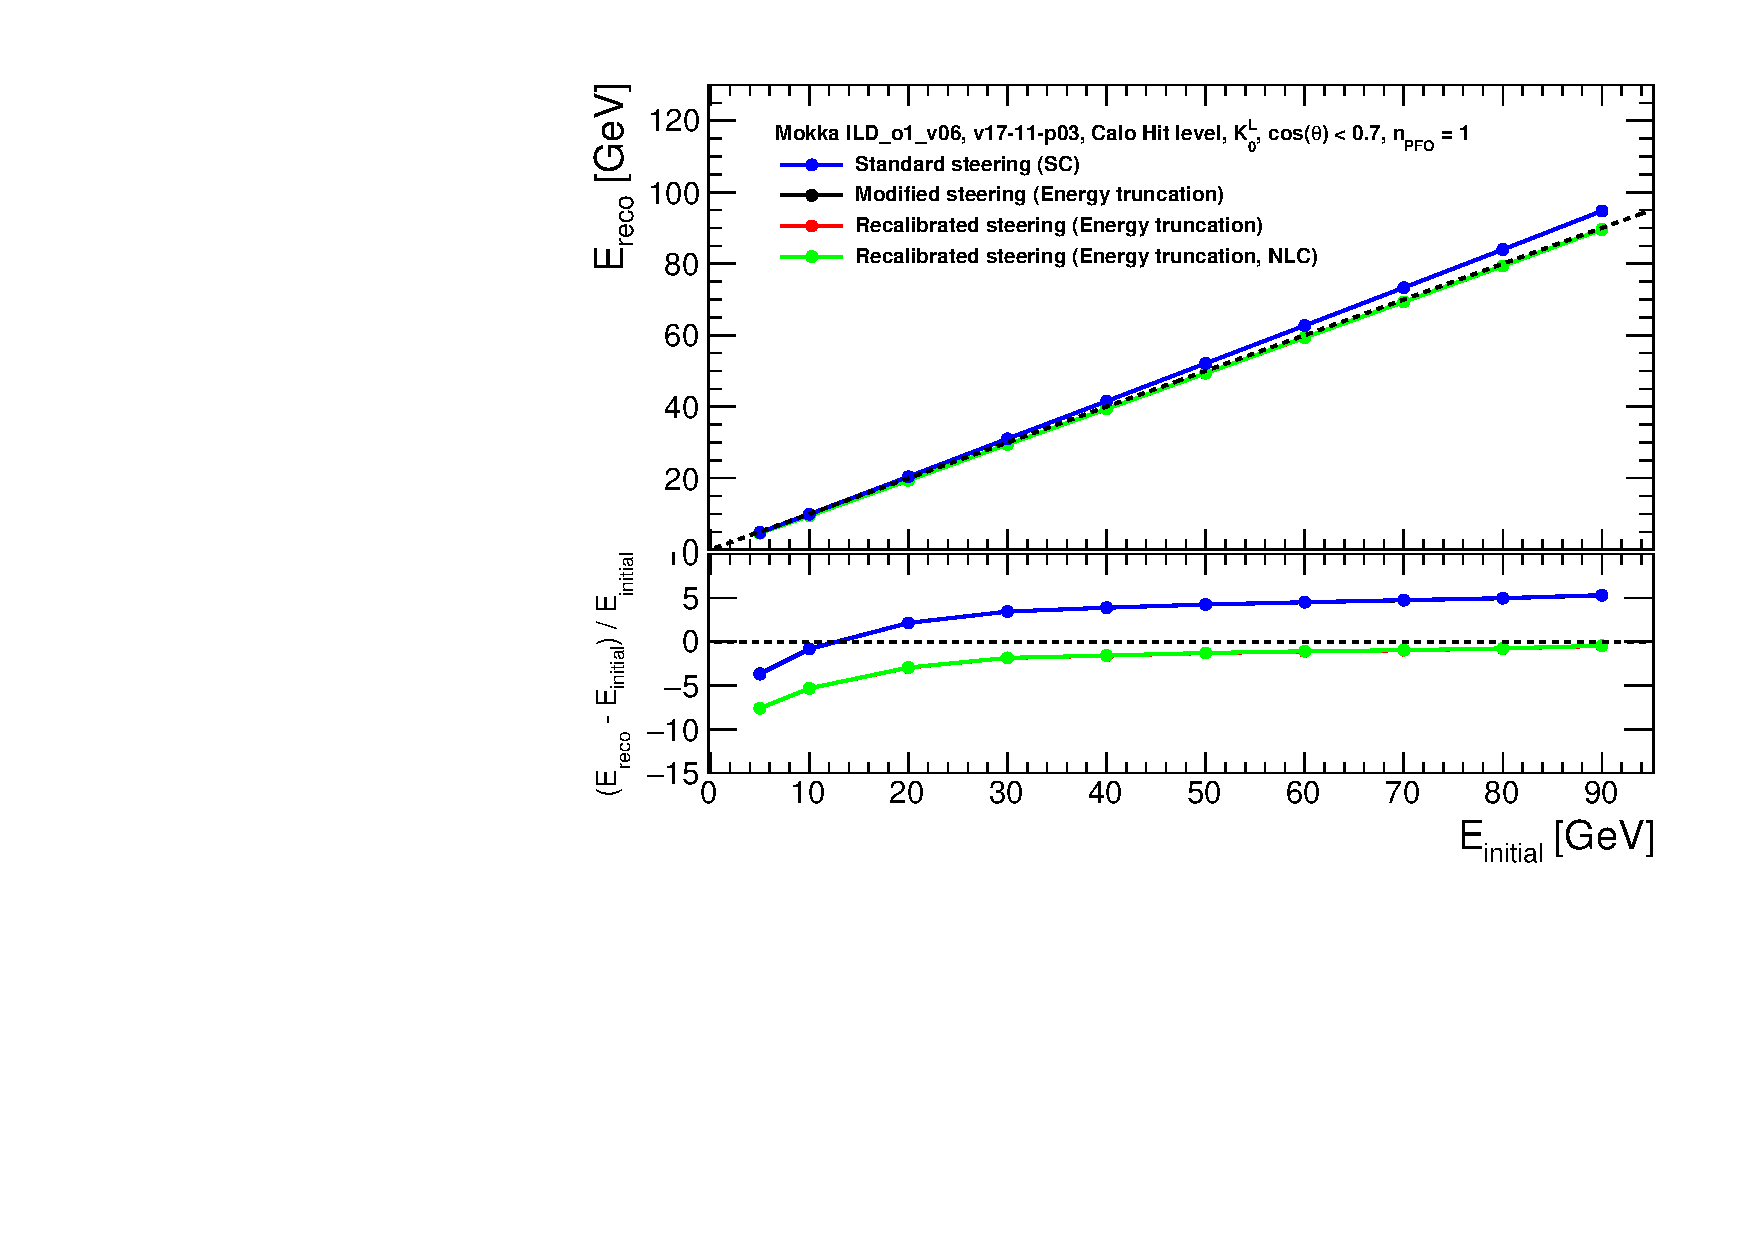
\includegraphics[width=1\linewidth]{chap6/fig_TimingILD/Comparison_linearity_Curves_Hits}
    \caption{Cluster hit linearity curve} \label{fig:linhits}
  \end{subfigure}
  \hfill
  \begin{subfigure}[t]{0.45\textwidth}
    \centering
    \raisebox{8ex}{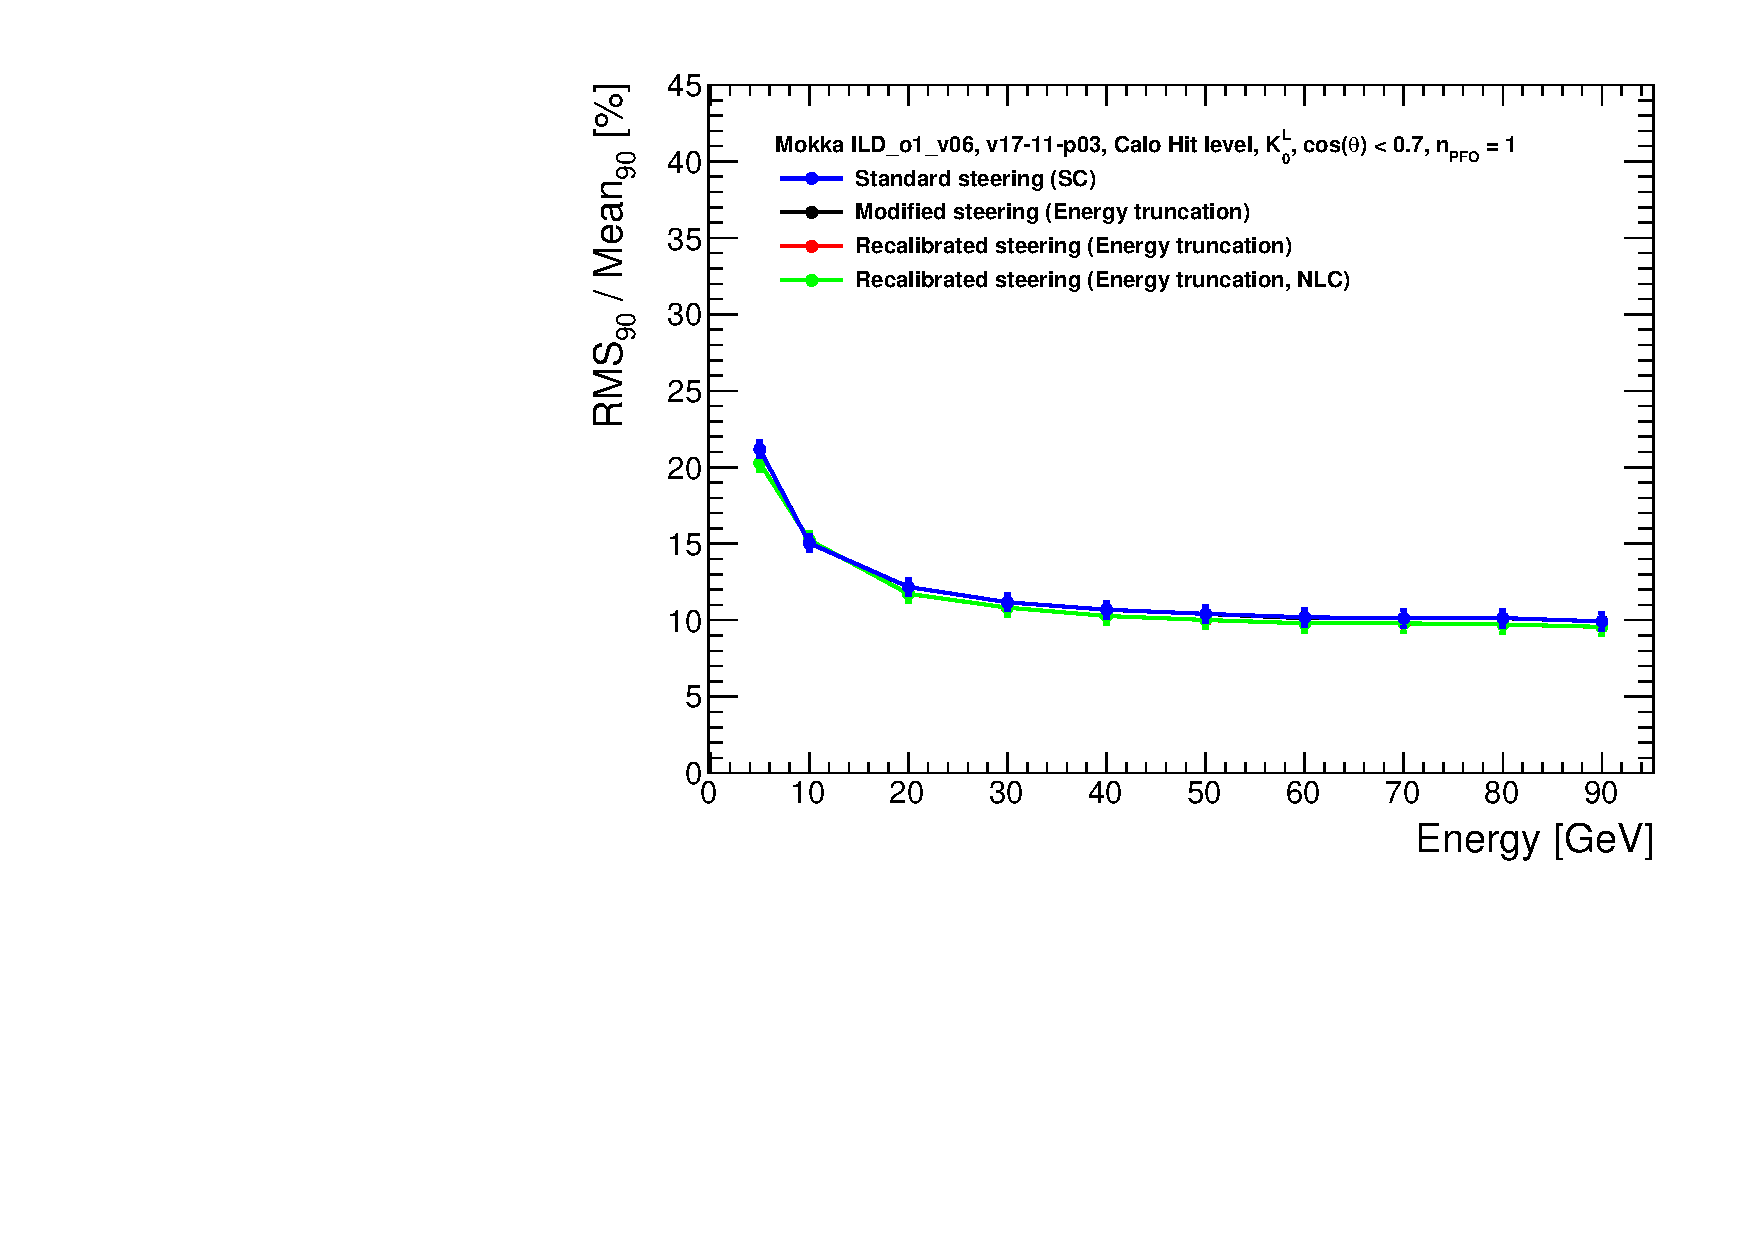
\includegraphics[width=1\linewidth]{chap6/fig_TimingILD/Comparison_resolution_Curves_Hits}}
    \caption{Cluster hit resolution curve} \label{fig:resohits}
  \end{subfigure}
  \caption{\subref{fig:linhits}) The top plot shows the mean reconstructed energy $E_{reco}$ for 5 to 90 GeV \kzeroL{} function of the simulated energy $E_{initial}$ for different constant parameters used in the reconstruction at the cluster hit level. The bottom plot shows the relative difference of the different curves to the line $x = y$. \subref{fig:resohits}) The plot shows the relative resolution RMS$_{90}$/Mean$_{90}$ for different constant parameters used in the reconstruction function of the energy. The blue curve uses the standard calibration, the black curve uses a modified set of parameters using energy truncation and no SC, the red curve uses constant parameters after recalibration and the green curve uses the same parameters as the red curve with non-linearity correction. The error bars represent statistical uncertainties.}
\end{figure}

Another option is to look at the PFO level as shown in figures \ref{fig:linpfo} and \ref{fig:resopfo}. This permits to understand the effects of the calibration constants in PandoraPFA.

The plots show a different picture. For the linearity curve, the red and black line are quite similar and show a non-lineariy especially at high energies between -10\% and 2\%. The green line is nicely linear thanks to the non-linearity correction. Then the blue line is off by around 10\%, this is believed to be due to the weights of the software conpensation that are not optimal for this model.

For the resolution curves, one can see a rise of the resolution at high energies for the red, green and black lines certainly due to the non-linearity. The blue curve present a bump after 50 GeV changing suddently the slope of the curve due to the over-correction of the energy.\\

\begin{figure}[t]
  \centering
  \begin{subfigure}[t]{0.45\textwidth}
    \centering
    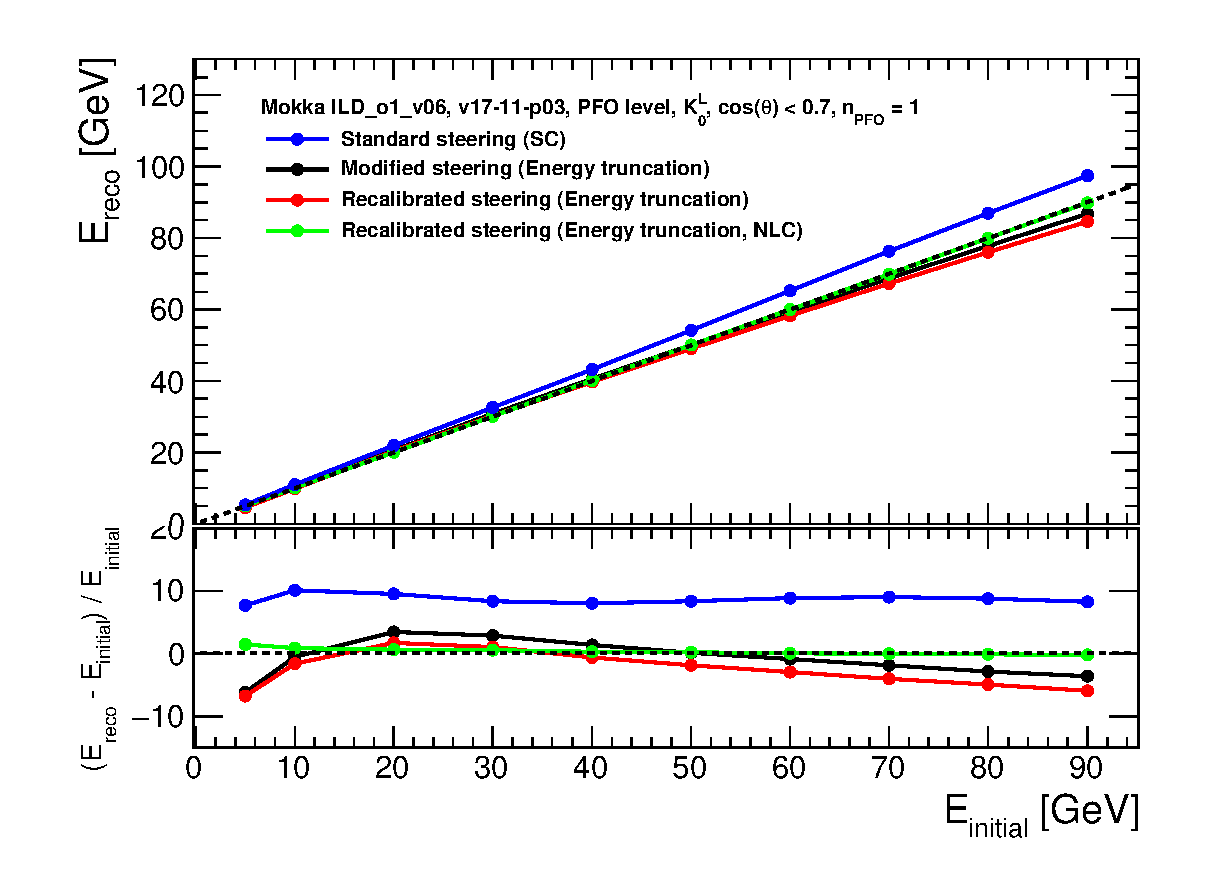
\includegraphics[width=1\linewidth]{chap6/fig_TimingILD/Comparison_linearity_Curves_PFO}
    \caption{PFO linearity curve} \label{fig:linpfo}
  \end{subfigure}
  \hfill
  \begin{subfigure}[t]{0.45\textwidth}
    \centering
    \raisebox{8ex}{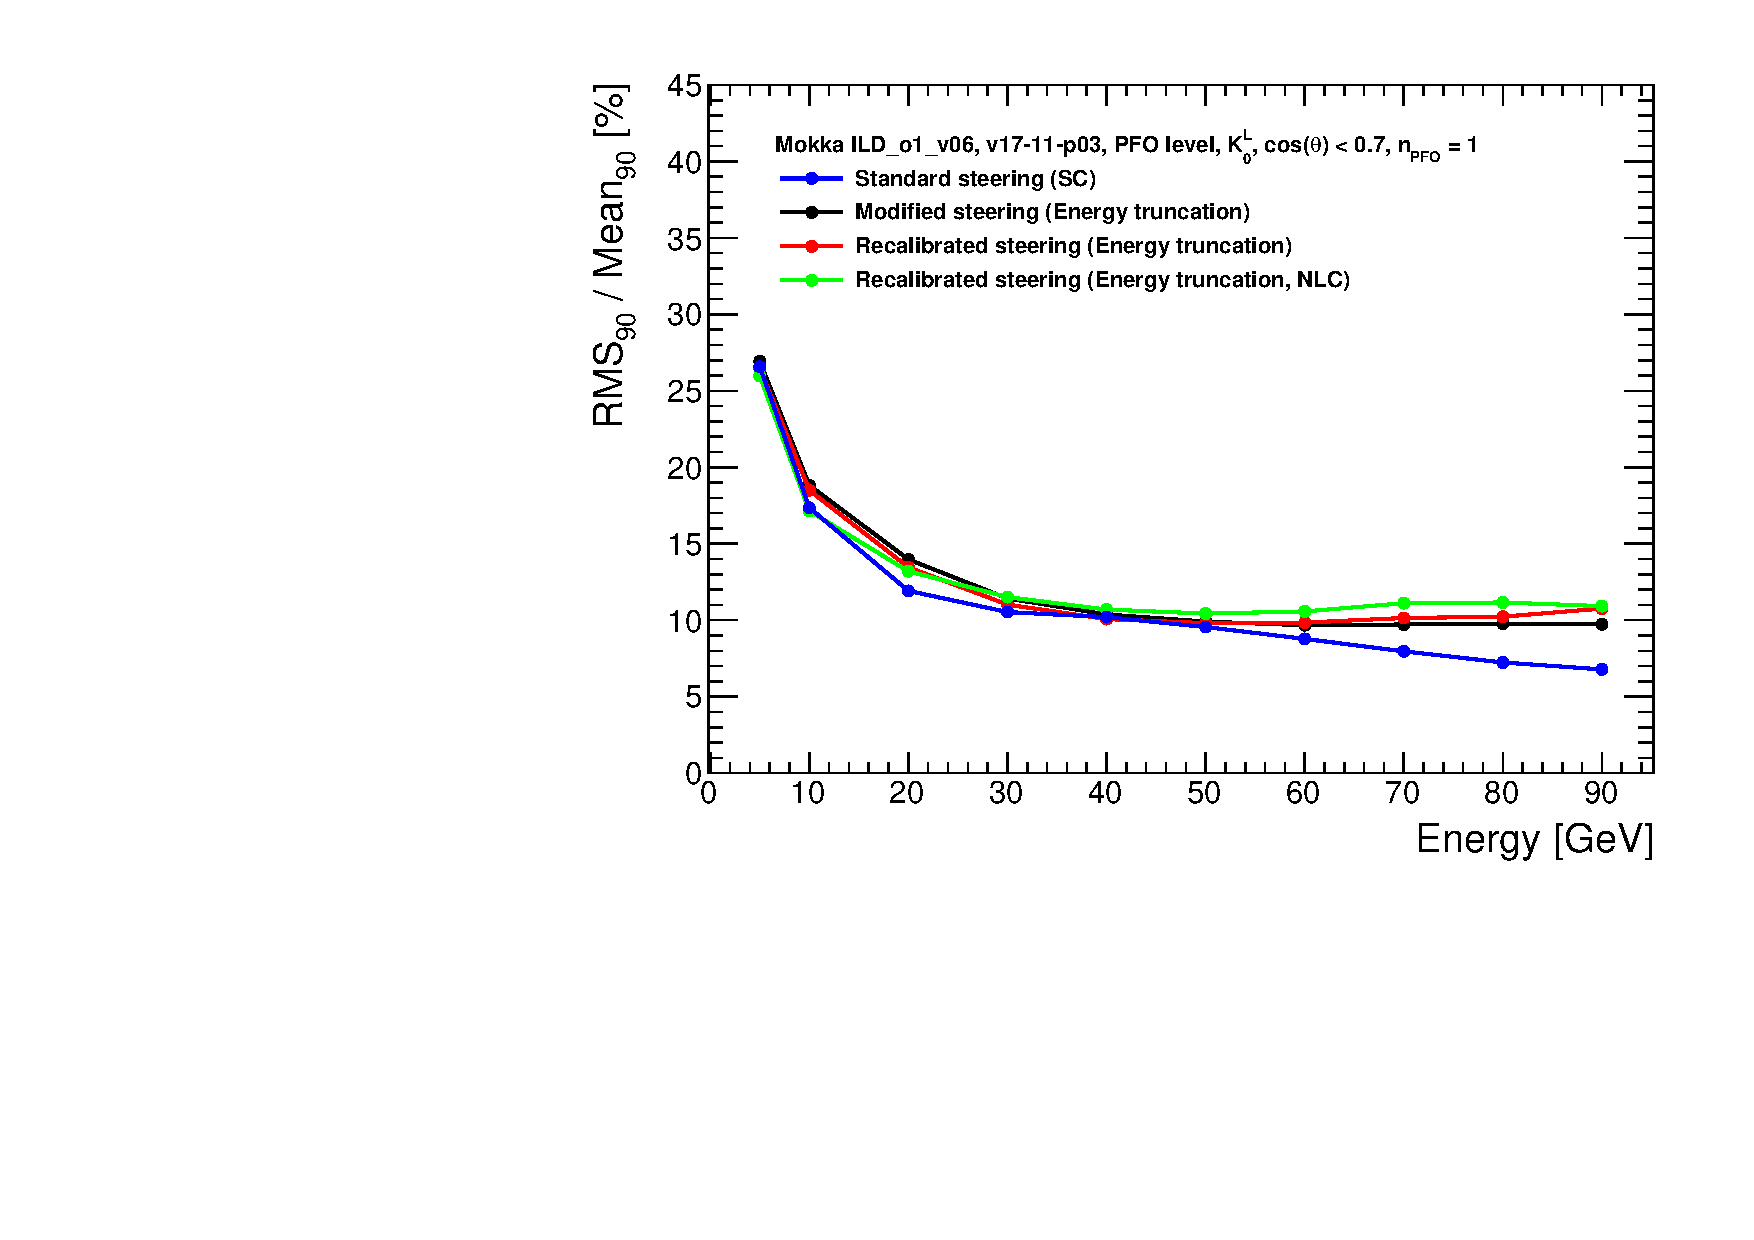
\includegraphics[width=1\linewidth]{chap6/fig_TimingILD/Comparison_resolution_Curves_PFO}}
    \caption{PFO resolution curve} \label{fig:resopfo}
  \end{subfigure}
  \caption{\subref{fig:linhits}) The top plot shows the mean reconstructed energy $E_{reco}$ for 5 to 90 GeV \kzeroL{} function of the simulated energy $E_{initial}$ for different constant parameters used in the reconstruction at the PFO level. The bottom plot shows the relative difference of the different curves to the line $x = y$. \subref{fig:resohits}) The plot shows the relative resolution RMS$_{90}$/Mean$_{90}$ for different constant parameters used in the reconstruction function of the energy. The blue curve uses the standard calibration, the black curve uses a modified set of parameters using energy truncation and no SC, the red curve uses constant parameters after recalibration and the green curve uses the same parameters as the red curve with non-linearity correction. The error bars represent statistical uncertainties.}
\end{figure}

Through the linearity is not perfect over all energies, the most regarded observable is the jet energy resolution. As explained in \ref{}, jets are mostly composed of charged particles of around 60\%. In this case, the energy of the PFO is coming from the track. Moreover neutral particles are counting in general for around 30\% of the contribution in a jet.

As shown in figure \ref{fig:momentumparticlejets}, for jets representative of heavy boson decay near production threshold, the momentum spectrum is dominant at around 10 \GeV as for heavy boosted jets with a more complex event topology, the momentum distribution is still dominant to low energies but present a tail to much higher energies. Thus the non-linearity has only little effect there. It is still relevant to understand the different effects of the reconstruction at single particle level.

\begin{figure}[t]
  \centering
  \begin{subfigure}[t]{0.45\textwidth}
    \centering
    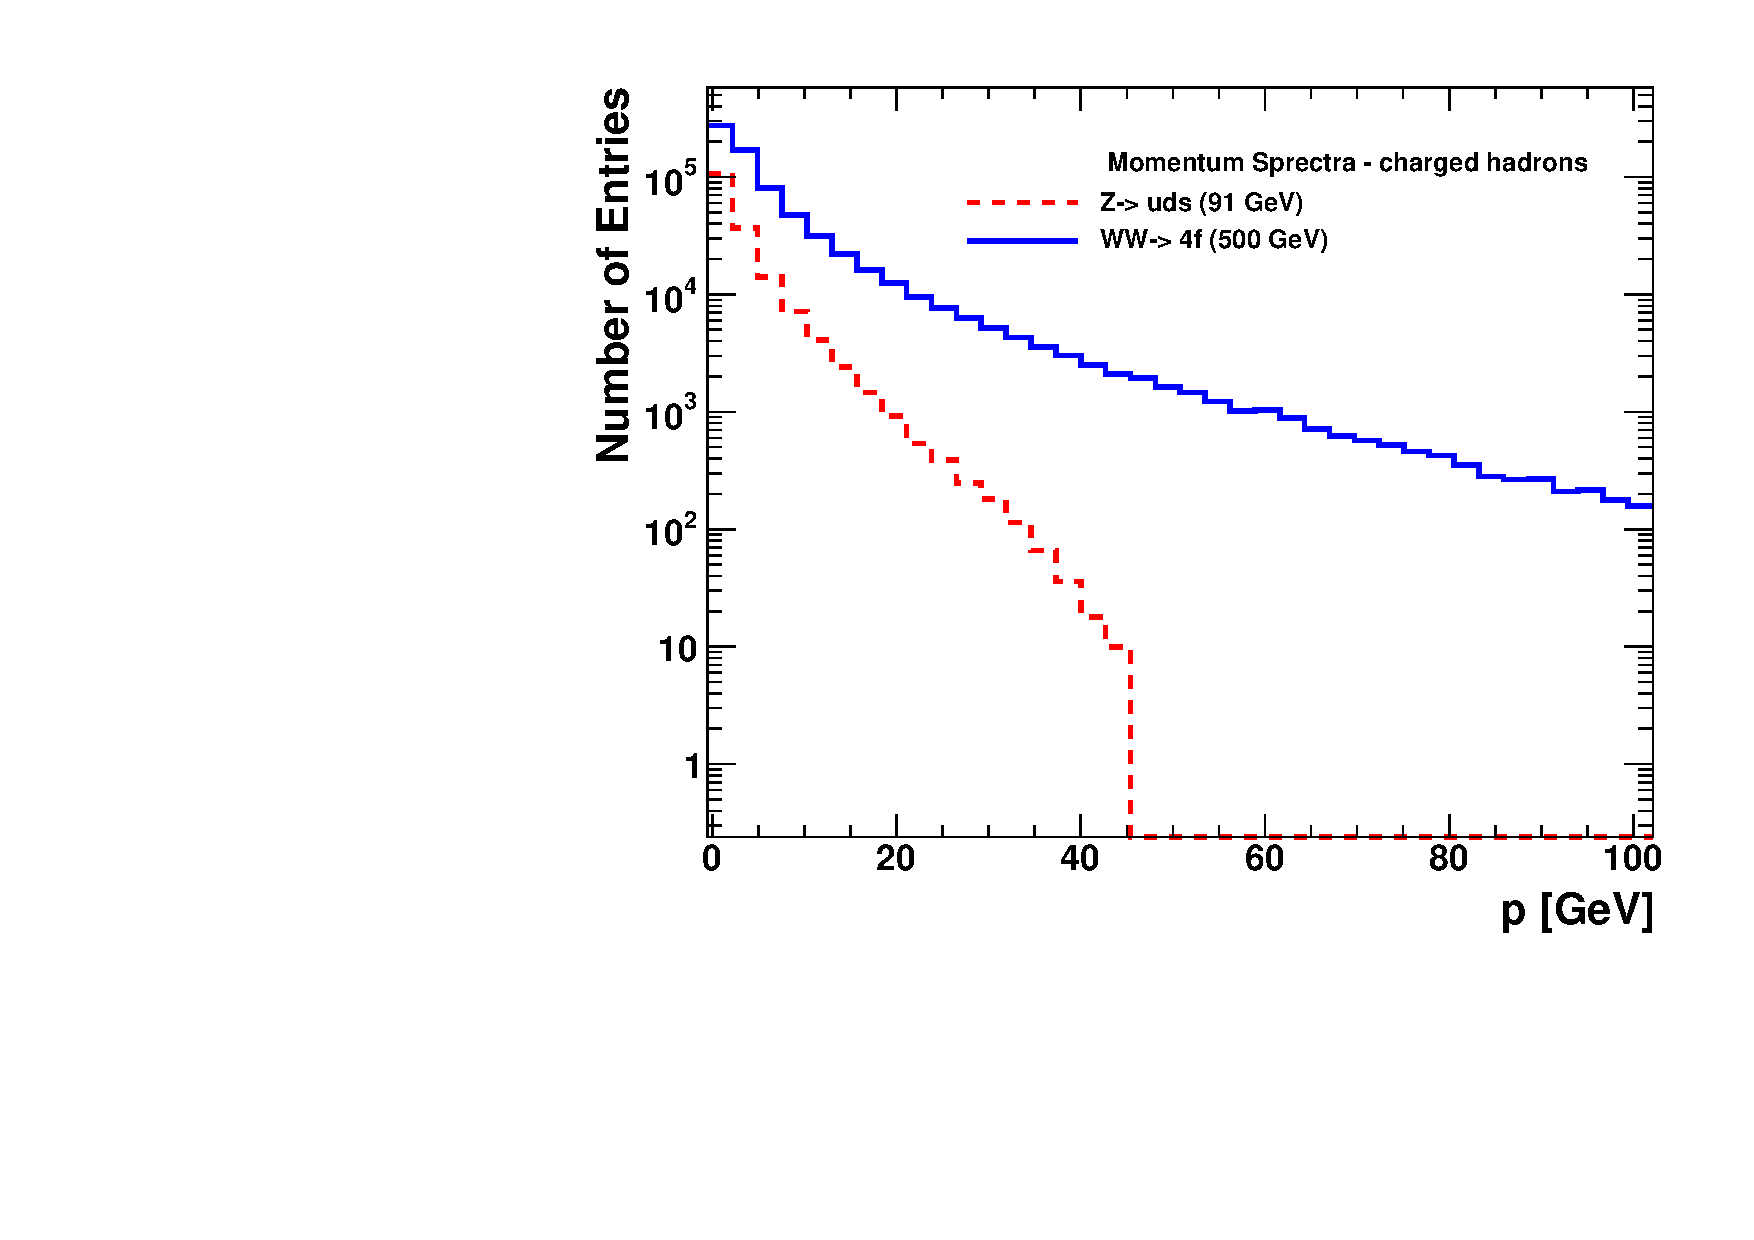
\includegraphics[width=1\linewidth]{chap6/fig_TimingILD/Momentum_spectra_to100GeV_final}
    \caption{Momentum spectrum of charged hadrons.} \label{fig:momentumparticlejets}
  \end{subfigure}
  \hfill
  \begin{subfigure}[t]{0.45\textwidth}
    \centering
    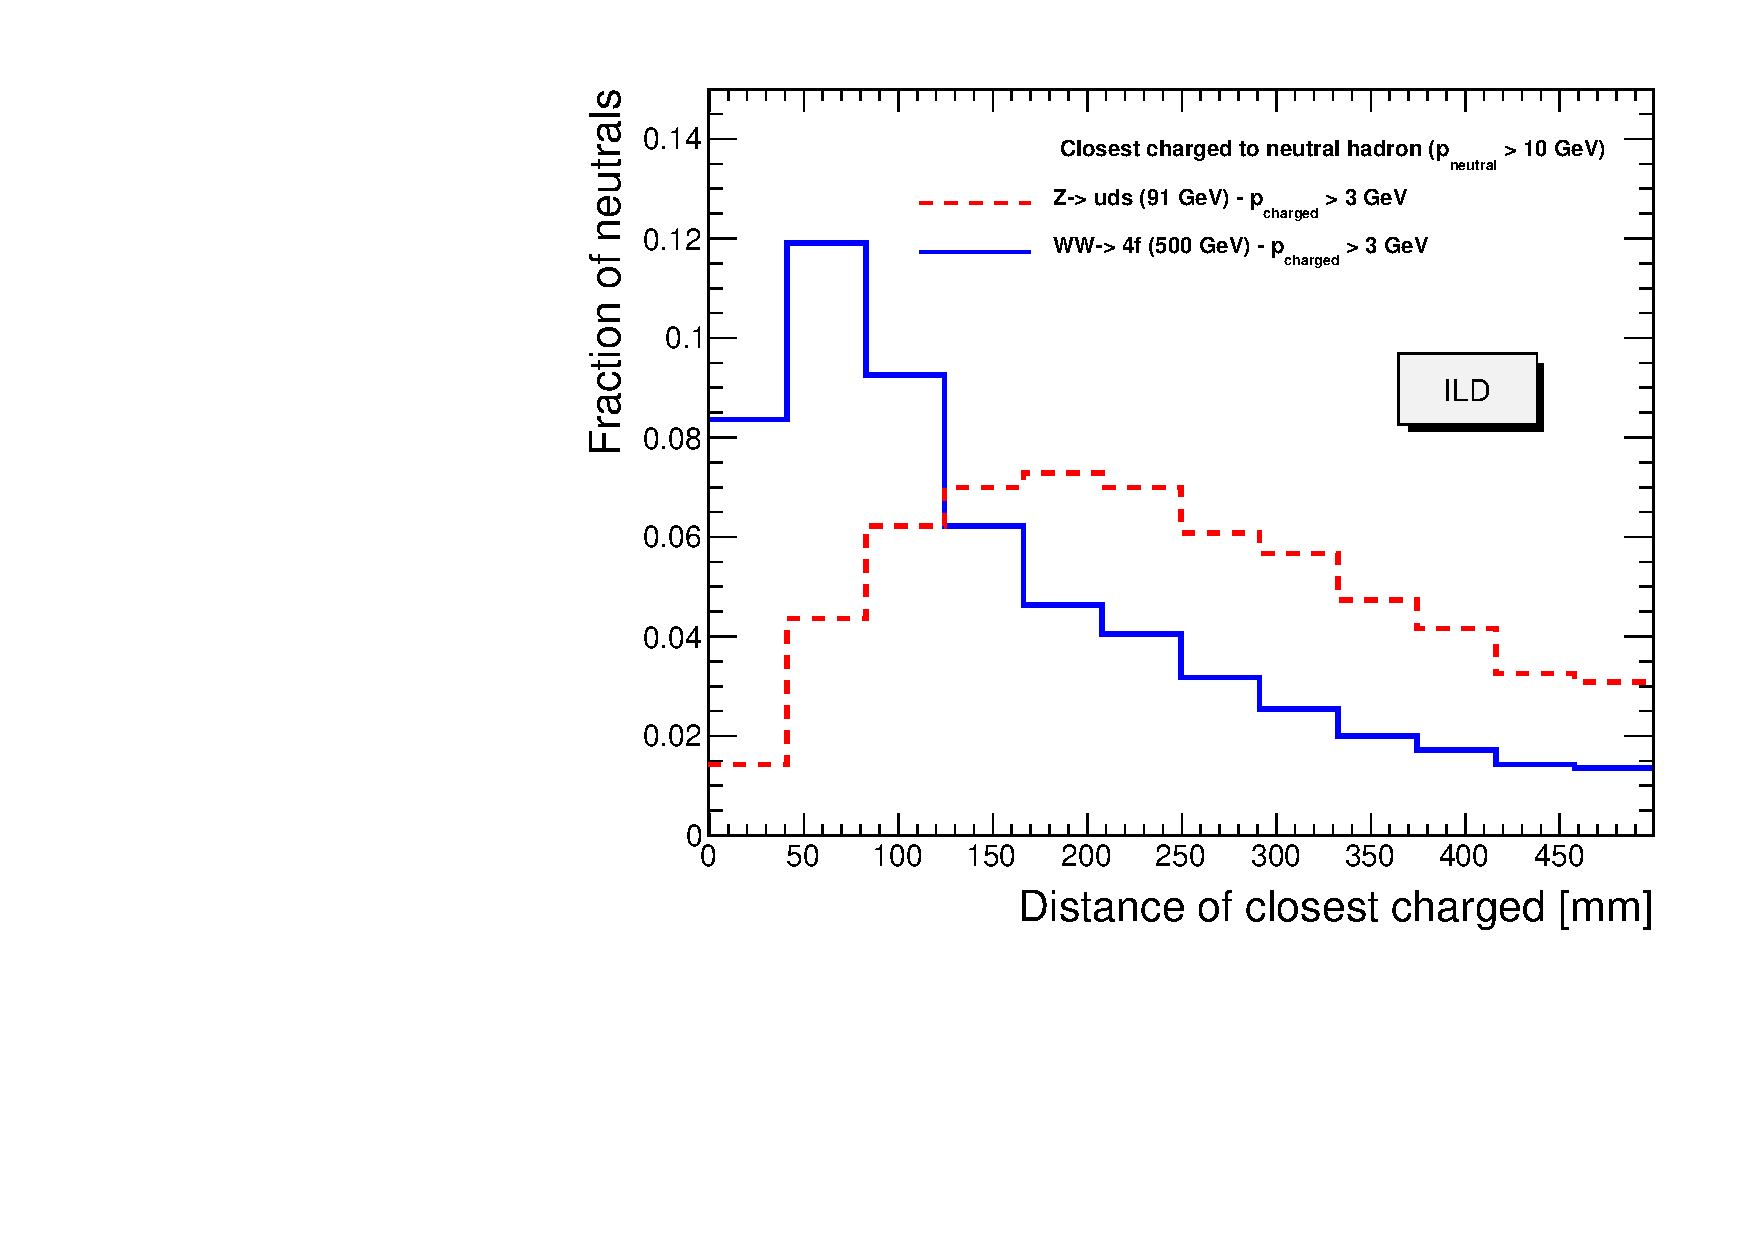
\includegraphics[width=1\linewidth]{chap6/fig_TimingILD/Stackall_dmin_3GeVneu_10GeVcharged_final_3_morestat}
    \caption{Minimal distance between a charged and neutral particle at the front face of the ECAL.} \label{fig:distancefrontfacejets}
  \end{subfigure}
  \caption{\subref{fig:momentumparticlejets}) Momentum distribution for charged particles in simulated \ee{}\ra{} \Zqq{} with $q = u,d,s$ at \rts{} = 91 \GeV and \ee{}\ra{} \WWqqqq{} where q is a quark at \rts{} = 500 \GeV. \subref{fig:distancefrontfacejets}) Distribution of distances to the closest charged track for neutral particles produced in \Zqq{} and \WWqqqq{} processes measured at the front face of the electromagnetic calorimeter in the ILD detector.}
\end{figure}

A complementary study was to look at the minimal distance between a charged and neutral particle for theses different physics processes. The figure \ref{fig:distancefrontfacejets} shows that for low energy jets the mean minimal distance (measured at the front face of the SiW-ECAL) between a charged and neutral hadron is around \SI{180}{\milli\meter} thus in this context, showers are well separated. But at higher energies where density is higher, typical distances of \SI{50}{\milli\meter} need to be resolved. This situation can become relevant in the contribution of confusion to the jet energy resolution. In this case, the use of timing information could help to separate nearby showers and improve the pattern recognition.

\subsection{Timing cut effects on hadronic showers in ILD detector}

In this section, the effect of timing cuts on hadronic showers is investigated. The study was performed using the \ilcsoft framework for reconstruction and a personal \marlin processor for analysis. In order to study the effect of timing on hadronic shower properties, the initial study was performed assuming a perfect timing resolution (i.e. the timing information is the Monte-Carlo truth). In a following step, several timing resolution were used to assess different scenarios. The smearing of the time was done by randomly sampling a normalised gaussian centered in \SI{0}{\nano\second} with a timing resolution denoted $\sigma_{t}$ = 0.4, 1 and \SI{8}{\nano\second}.

The selection of events is fairly simple, only events in the barrel region ($cos\theta < 0.7$) are selected. All the calorimeter hits in the ECAL and HCAL are used.

\subsubsection{On Monte-Carlo level}

The following section present results of timing cuts assuming a perfect time resolution. To avoid any effects of clustering and Pandora, the study was performed at the calorimeter hit level. Several shower observables were looked at as a function of the time cut for energies from 5 \GeV to 90 \GeV \kzeroL. The different time cuts used are: 1, 2, 3, 5, 8, 10, 15, 20, 25, 30, 50, 70 and \SI{100}{\nano\second}.

The figures \ref{fig:linearityNoSmearing} and \ref{fig:resoNoSmearing} show the effect of timing cut on linearity and energy resolution. The tighter the timing cut gets, the linearity and resolution gets degraded. This effectively means that with a harder timing cut more hits of the shower are removed but mostly only outer hits carrying only a small fraction of the total shower energy, the core of the shower mostly does not get affected by timing cut up to few nanoseconds.

\begin{figure}[t]
  \centering
  \begin{subfigure}[t]{0.45\textwidth}
    \centering
    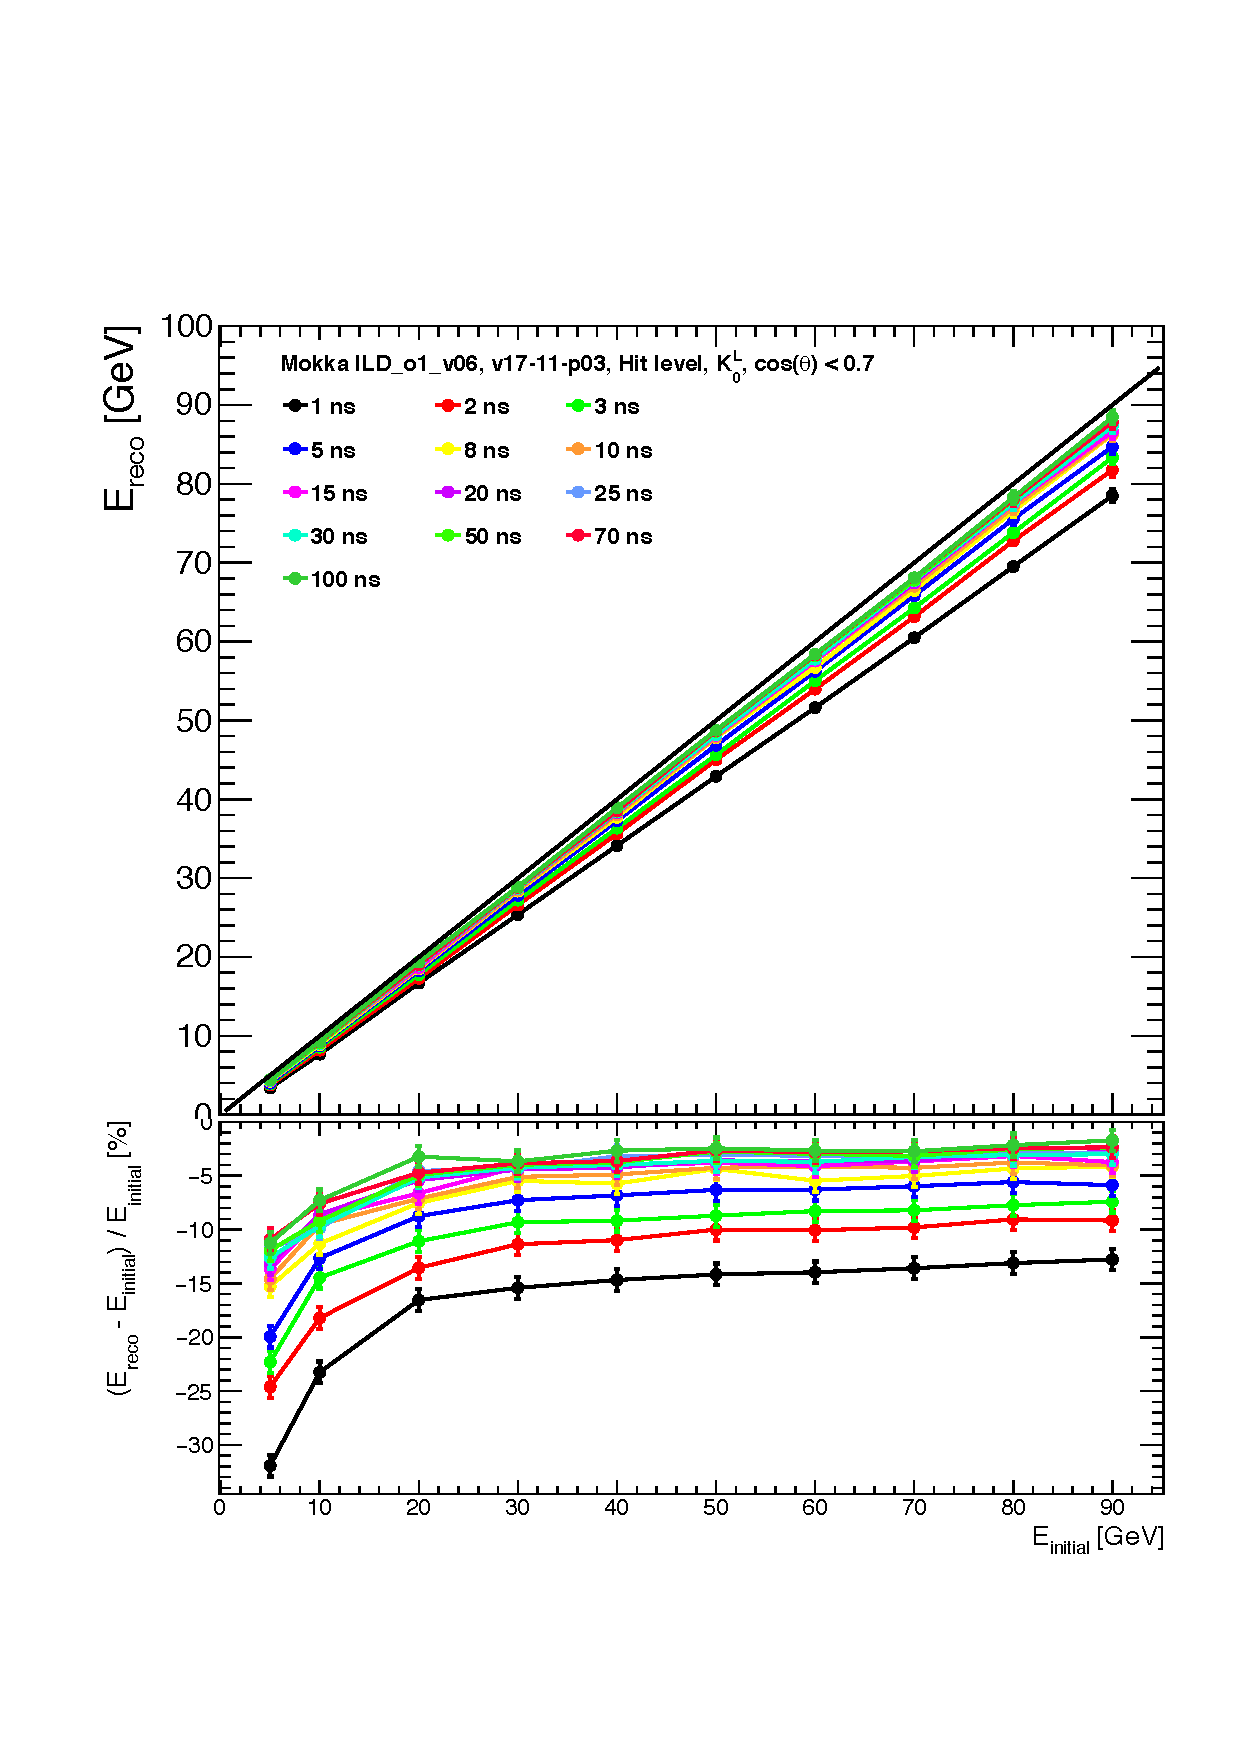
\includegraphics[width=1\linewidth]{chap6/fig_TimingILD/NoSmearing/Linearity_TimeCuts_noSmearing}
    \caption{Linearity curve with no time smearing.} \label{fig:linearityNoSmearing}
  \end{subfigure}
  \hfill
  \begin{subfigure}[t]{0.45\textwidth}
    \centering
    \raisebox{8ex}{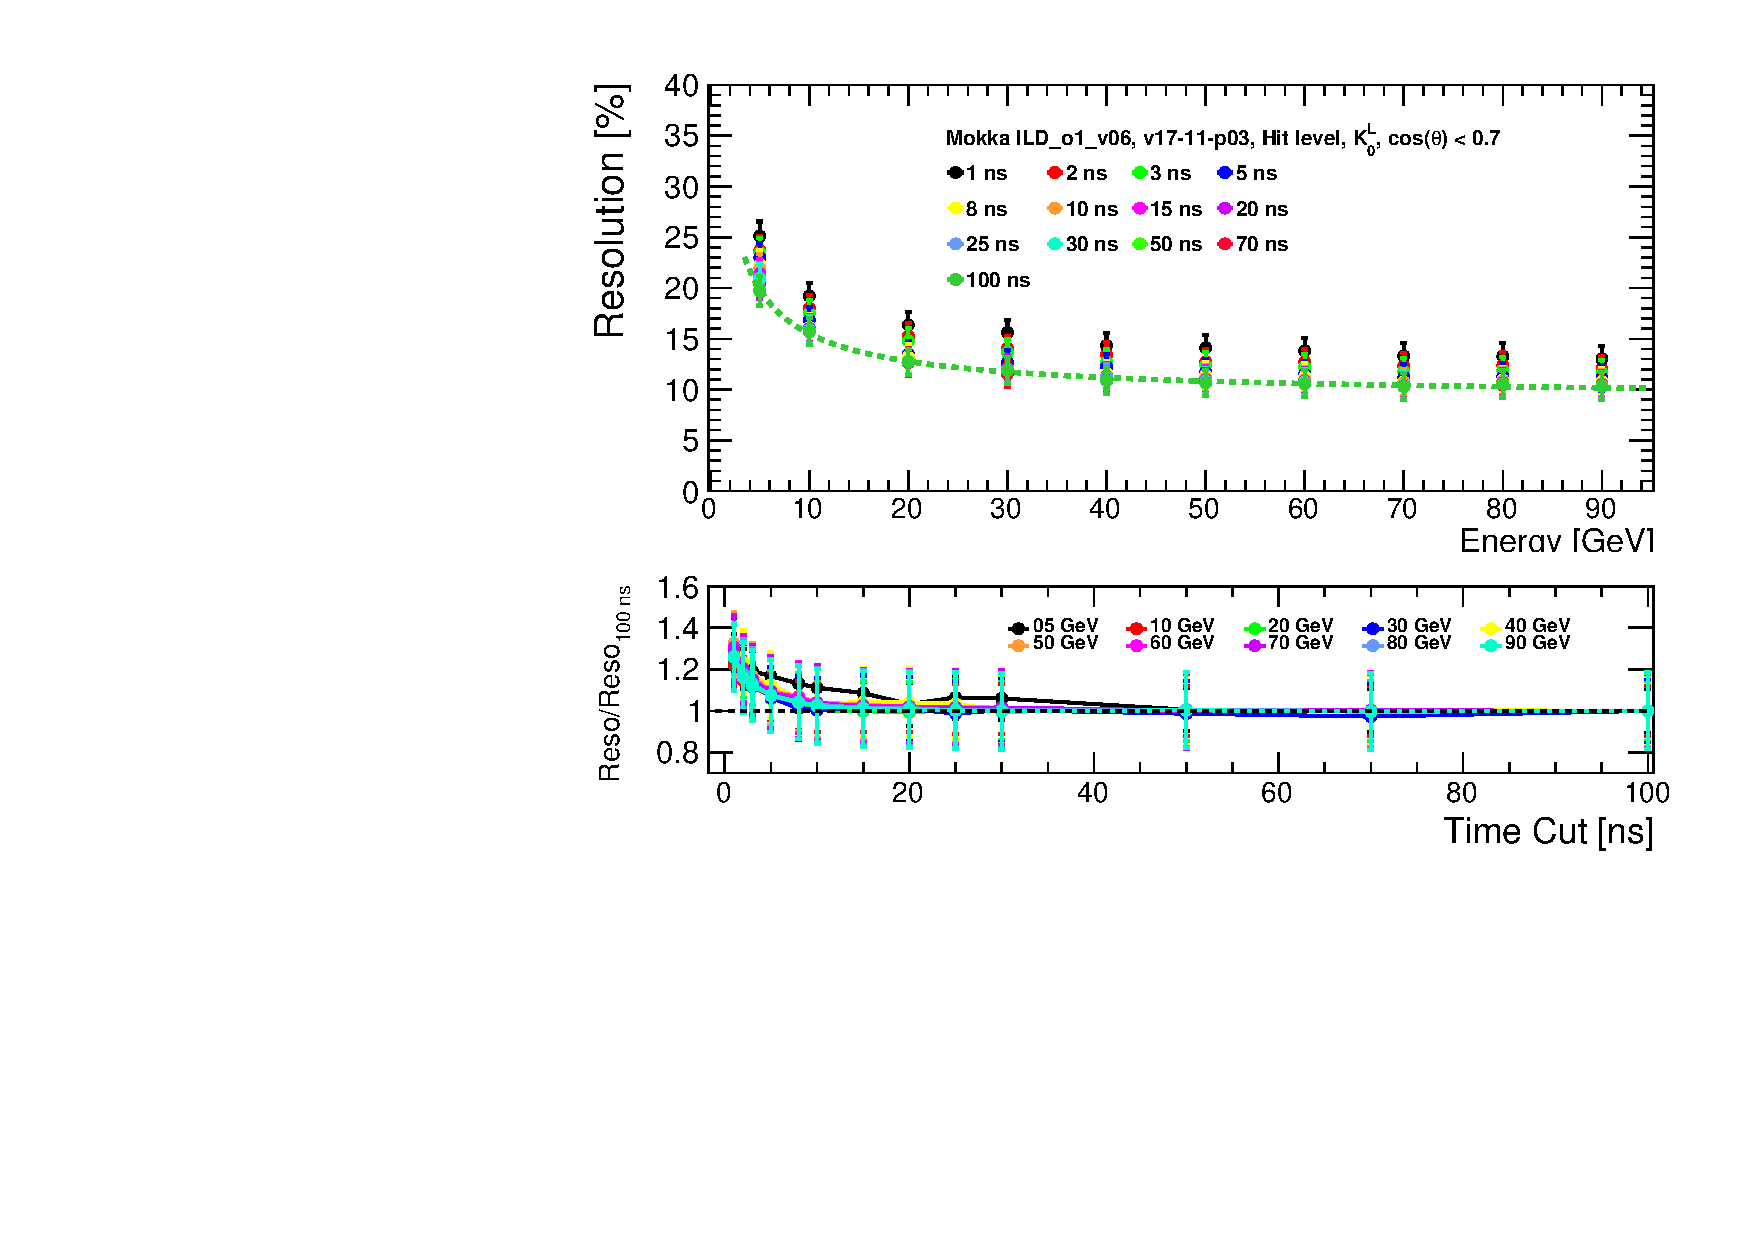
\includegraphics[width=1\linewidth]{chap6/fig_TimingILD/NoSmearing/ShowerResoAbsolute_TimeCuts_noSmearing}}
    \caption{Resolution curve with no time smearing.} \label{fig:resoNoSmearing}
  \end{subfigure}
  \caption{\subref{fig:linearityNoSmearing}) The top plot represent the linearity curve in the ILD detector over a range of energy from 5 \GeV to 90 \GeV for different timing cuts assuming a perfect resolution. The bottom plot represent the relative deviation to the line $x=y$ for the different time cuts. \subref{fig:resoNoSmearing}) The plot illustrates the relative energy resolution ($\frac{\sigma_{E}}{E}$) at single particle level for different timing cuts. The green line is a fit performed at \SI{100}{\nano\second} of the form $\frac{\sigma_{E}}{E} = \frac{a}{\sqrt{E}} \bigoplus b$ where $a$ is the stochastic term ($44.01\% \pm 3.17$) and $b$ the constant term ($7.26 \pm 0.84$).}
\end{figure}

The figure \ref{fig:resoRelativeNoSmearing} shows the relative impact on the energy resolution compared to the \SI{100}{\nano\second} cut as function of timing cuts for all energies. The energy resolution is mostly not affected over a cut of around \SI{20}{\nano\second} meaning that the removed hits are not carrying a lot of energy and are part of the shower halo. Then below \SI{20}{\nano\second}, the resolution starts to degrade slowly relatively in the same way for all energies. A hard cut of 1 ns will degrade greatly the energy resolution up to around 30\%.

\begin{figure}[t]
  \centering
  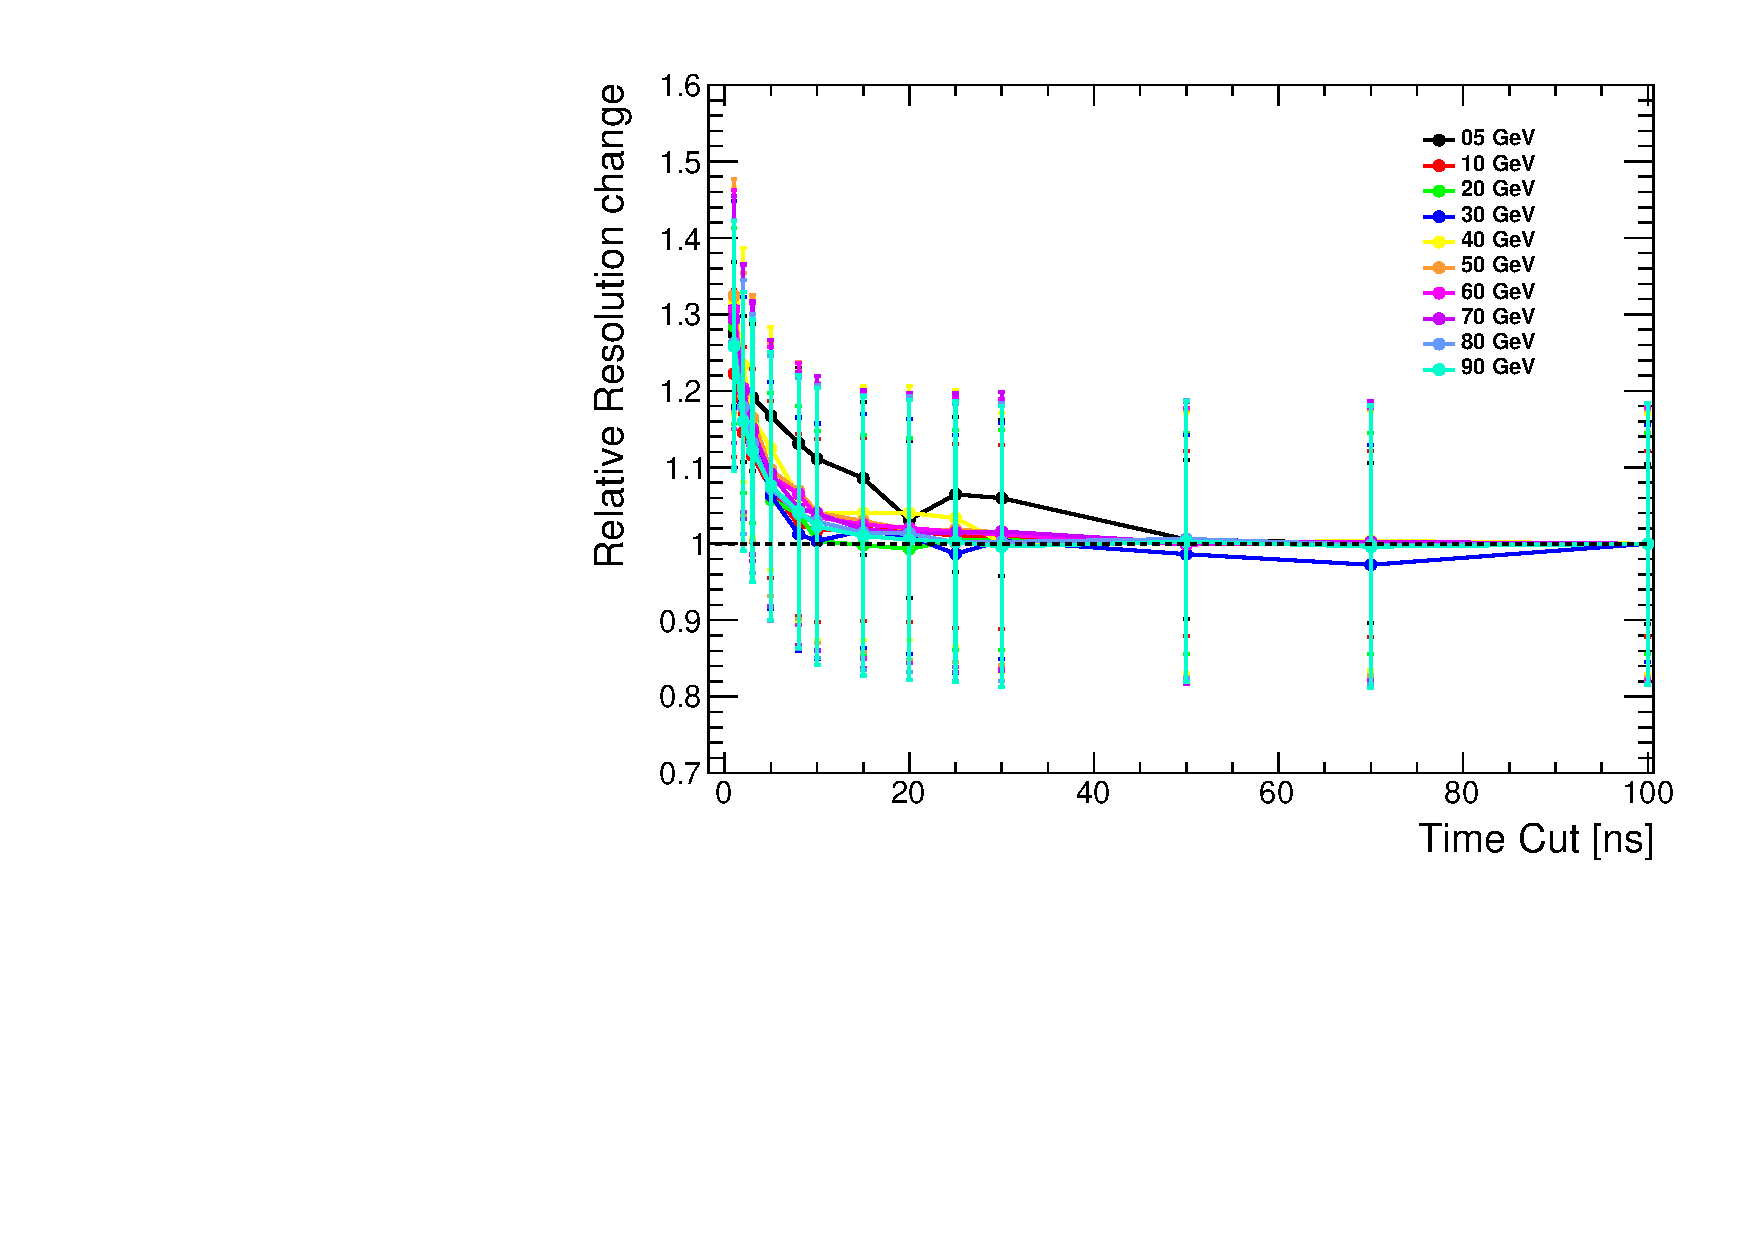
\includegraphics[width=0.5\linewidth]{chap6/fig_TimingILD/NoSmearing/ShowerReso_TimeCuts_noSmearing}
  \caption{Relative change of the energy resolution compared to \SI{100}{\nano\second} as function of the timing cut. The error bars represent the statistical uncertainty.} \label{fig:resoRelativeNoSmearing}
\end{figure}

The figure \ref{RadialProfNoSmearing} shows the radial profile of a 50 \GeV hadronic shower. The radial profile of the shower is filled for each hit with the distance to the main shower axis ($R_{i}$, eq.\ref{eq:radialprof})  weighted by the hit energy ($E_{i}$).

\begin{equation} \label{eq:radialprof}
  \begin{split}
    & R_{i} = \sqrt{\Sigma_{i} (r_{i} - r_{cog})^{2} - \lVert (\mathbf{r_{i}} - \mathbf{r_{cog}}) \cdot \mathbf{Eigen} \rVert^{2}}) \\
    & \text{with} \quad \mathbf{r_{i}} = (x_i, y_i, z_i) \quad \text{and} \quad \mathbf{r_{CoG}} = (cog_x, cog_y, cog_z)
  \end{split}
\end{equation}

The main part of the energy density is situated in the core within few centimeters. The influence of timing cuts is highly visible in the tail of the distribution (or halo of the shower) and as very little influence on the energy density deposited in core of the shower. Though an effect of increase of energy density in the two first bins of the distribution is visible. This effect is related to a displacement of the center of gravity (CoG) as function of the timing cut as outer hits of the shower are removed. This has been checked by looking at the hit radius distribution relative to a fixed reference instead of the CoG (the Monte-Carlo particle endpoint) as shown in figure \ref{fig:HitRadiusSmearing}. One can observe that in this case, the timing cut removes only part of the tail and does not affect the core of the distribution.

\begin{figure}[t]
  \centering
  \begin{subfigure}[t]{0.45\textwidth}
    \centering
    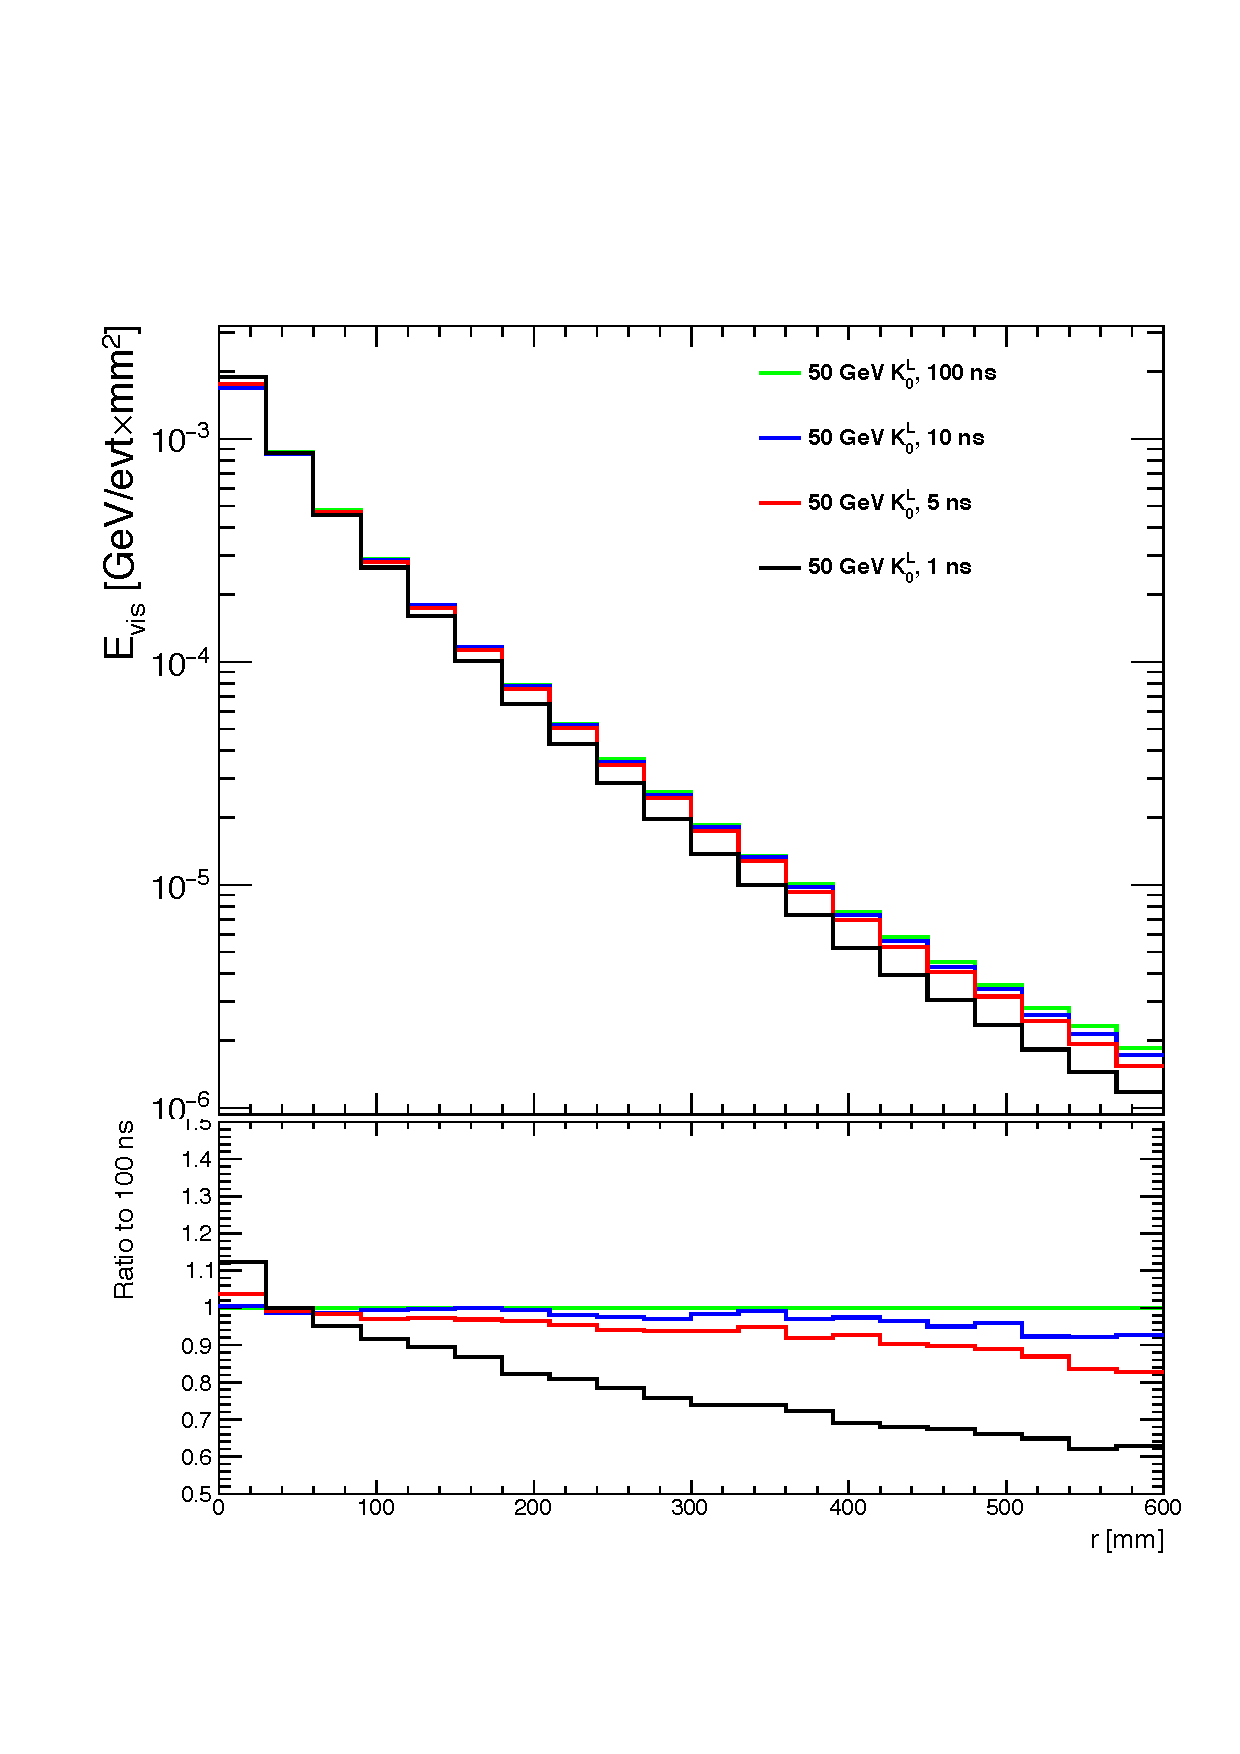
\includegraphics[width=1\linewidth]{chap6/fig_TimingILD/NoSmearing/RadialProfileOverlay_noSmearing}
    \caption{Radial profile.} \label{fig:RadialProfNoSmearing}
  \end{subfigure}
  \hfill
  \begin{subfigure}[t]{0.45\textwidth}
    \centering
    \raisebox{8ex}{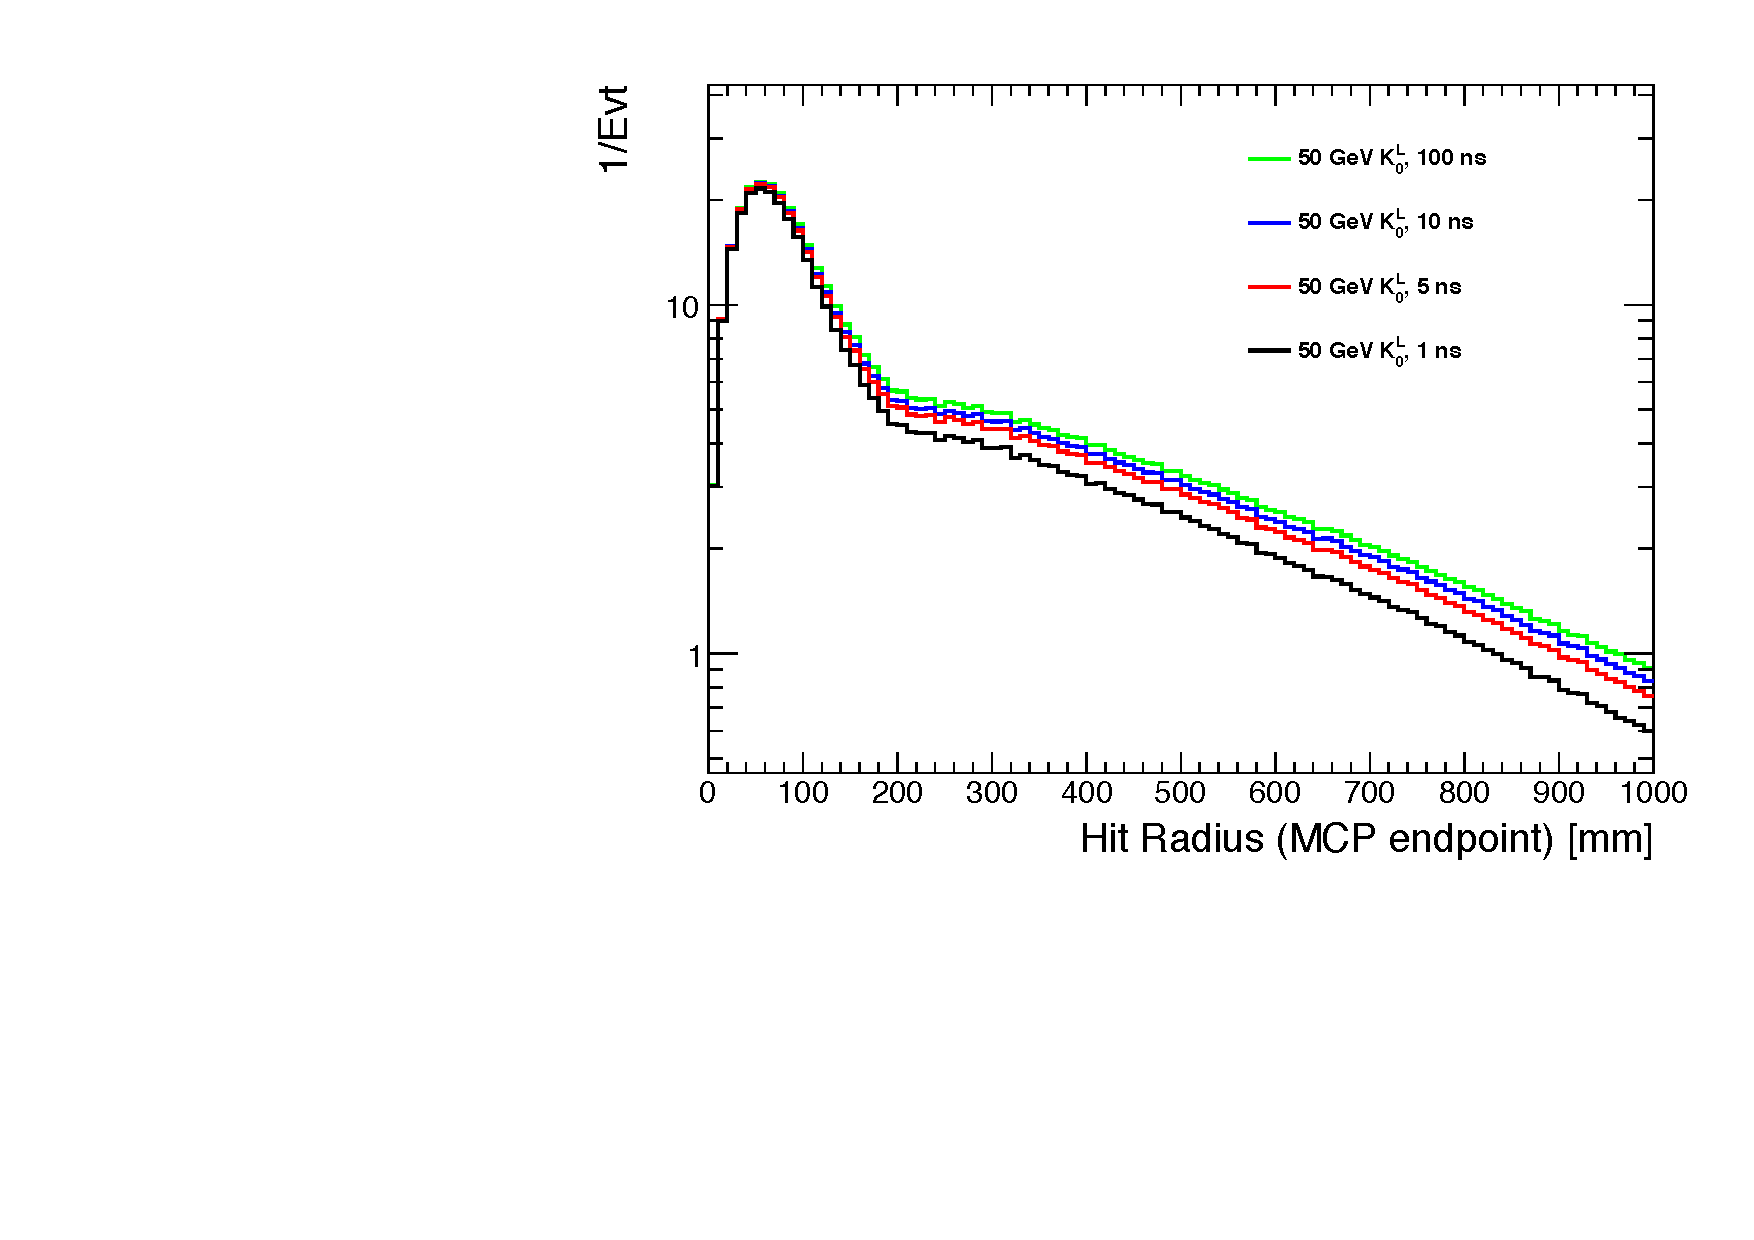
\includegraphics[width=1\linewidth]{chap6/fig_TimingILD/NoSmearing/HitRadiusOverlayMCP_TimeCuts_noSmearing}}
    \caption{Hit radius.} \label{fig:HitRadiusSmearing}
  \end{subfigure}
  \caption{\subref{fig:RadialProfNoSmearing}) The top plot shows the radial profile of a 50 \GeV hadronic shower overlayed for different timing cuts. The bottom plot shows the ratio of the histograms to \SI{100}{\nano\second} radial profile. \subref{fig:HitRadiusSmearing}) Hit radius histograms at 50 \GeV for different timing cuts.}
\end{figure}

Another aspect looked at was the influence of timing cut on the shower width <R> (eq.\ref{eq:showerwidth}) defined as:

\begin{equation} \label{eq:showerwidth}
  <R> = \frac{\Sigma_i E_i r_i}{\Sigma_i E_i}
\end{equation}
\vspace{1ex}

The figures \ref{fig:ShowerWidthNoSmearing} and \ref{fig:ShowerWidthAbsoNoSmearing} show the shower width <R> for different particle energies as function of the timing cut. It shows that a tight timing cut at\SI{1}{\nano\second} can reduce the shower width up to around 70\%. One can observe also that the shower width at 5 and 10 \GeV are behaving differently than higher than 10 \GeV. This may come from the transition from the Bertini model (BERT) to the quark string gluon model (QGSP) in the physics list in this energy range. Looking at the shower width in absolute value, hadronic showers are wider at lower energies ($\sim$\SI{180}{\milli\meter} for 5 \GeV) certainly due to the magnetic field. Applying a timing cut removes more and more hits from the halo of the shower, thus reducing its size up to a point where it reaches the core of the shower at $\sim$\SI{20}{\nano\second} timing cut where the shower is around a couple of tiles in size. At this point, the shower width behaves similarly for all energies by reducing gradually the size of the core.

\begin{figure}[t]
  \centering
  \begin{minipage}{.45\textwidth}
    \begin{subfigure}[t]{0.7\textwidth}
      \centering
      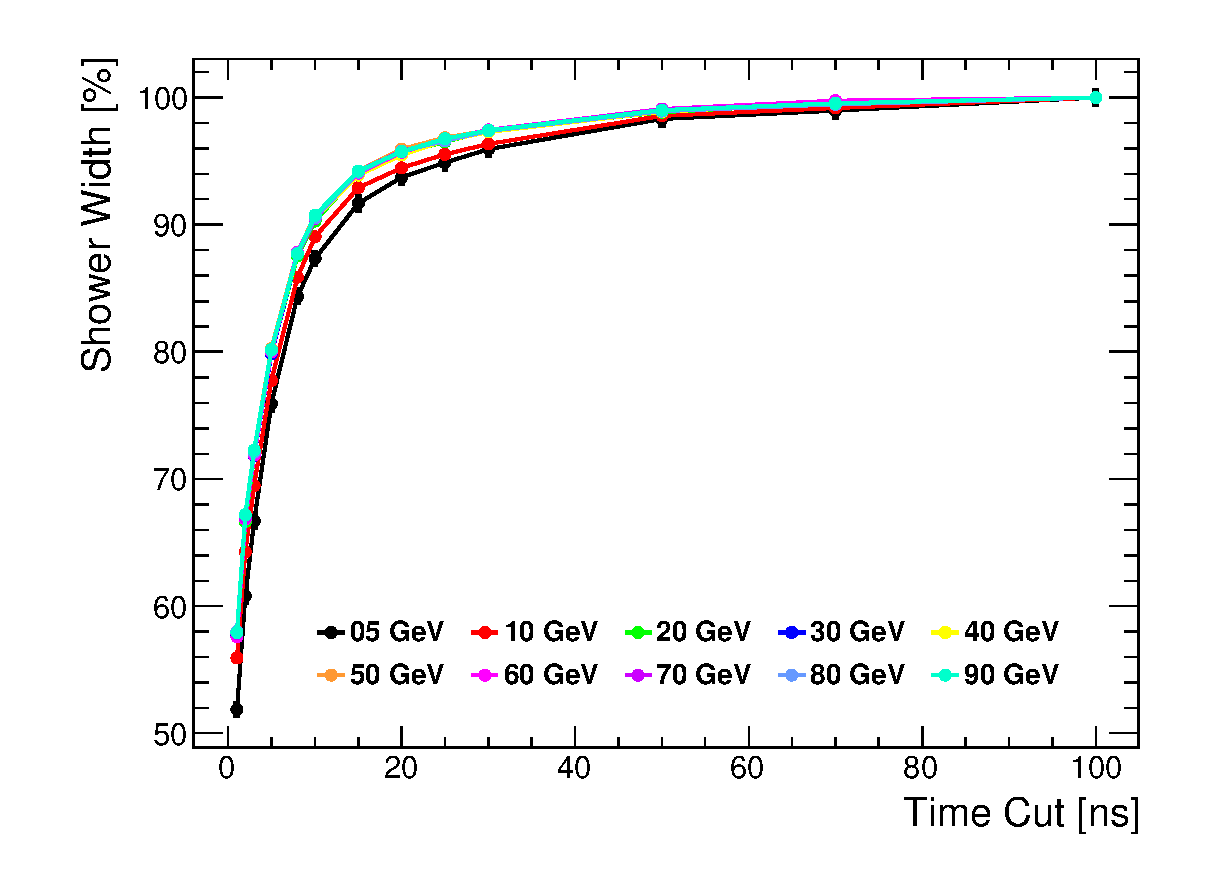
\includegraphics[width=1\linewidth]{chap6/fig_TimingILD/NoSmearing/ShowerWidth_TimeCuts_noSmearing}
      \caption{} \label{fig:ShowerWidthNoSmearing}
    \end{subfigure}
    \begin{subfigure}[t]{0.7\textwidth}
      \centering
      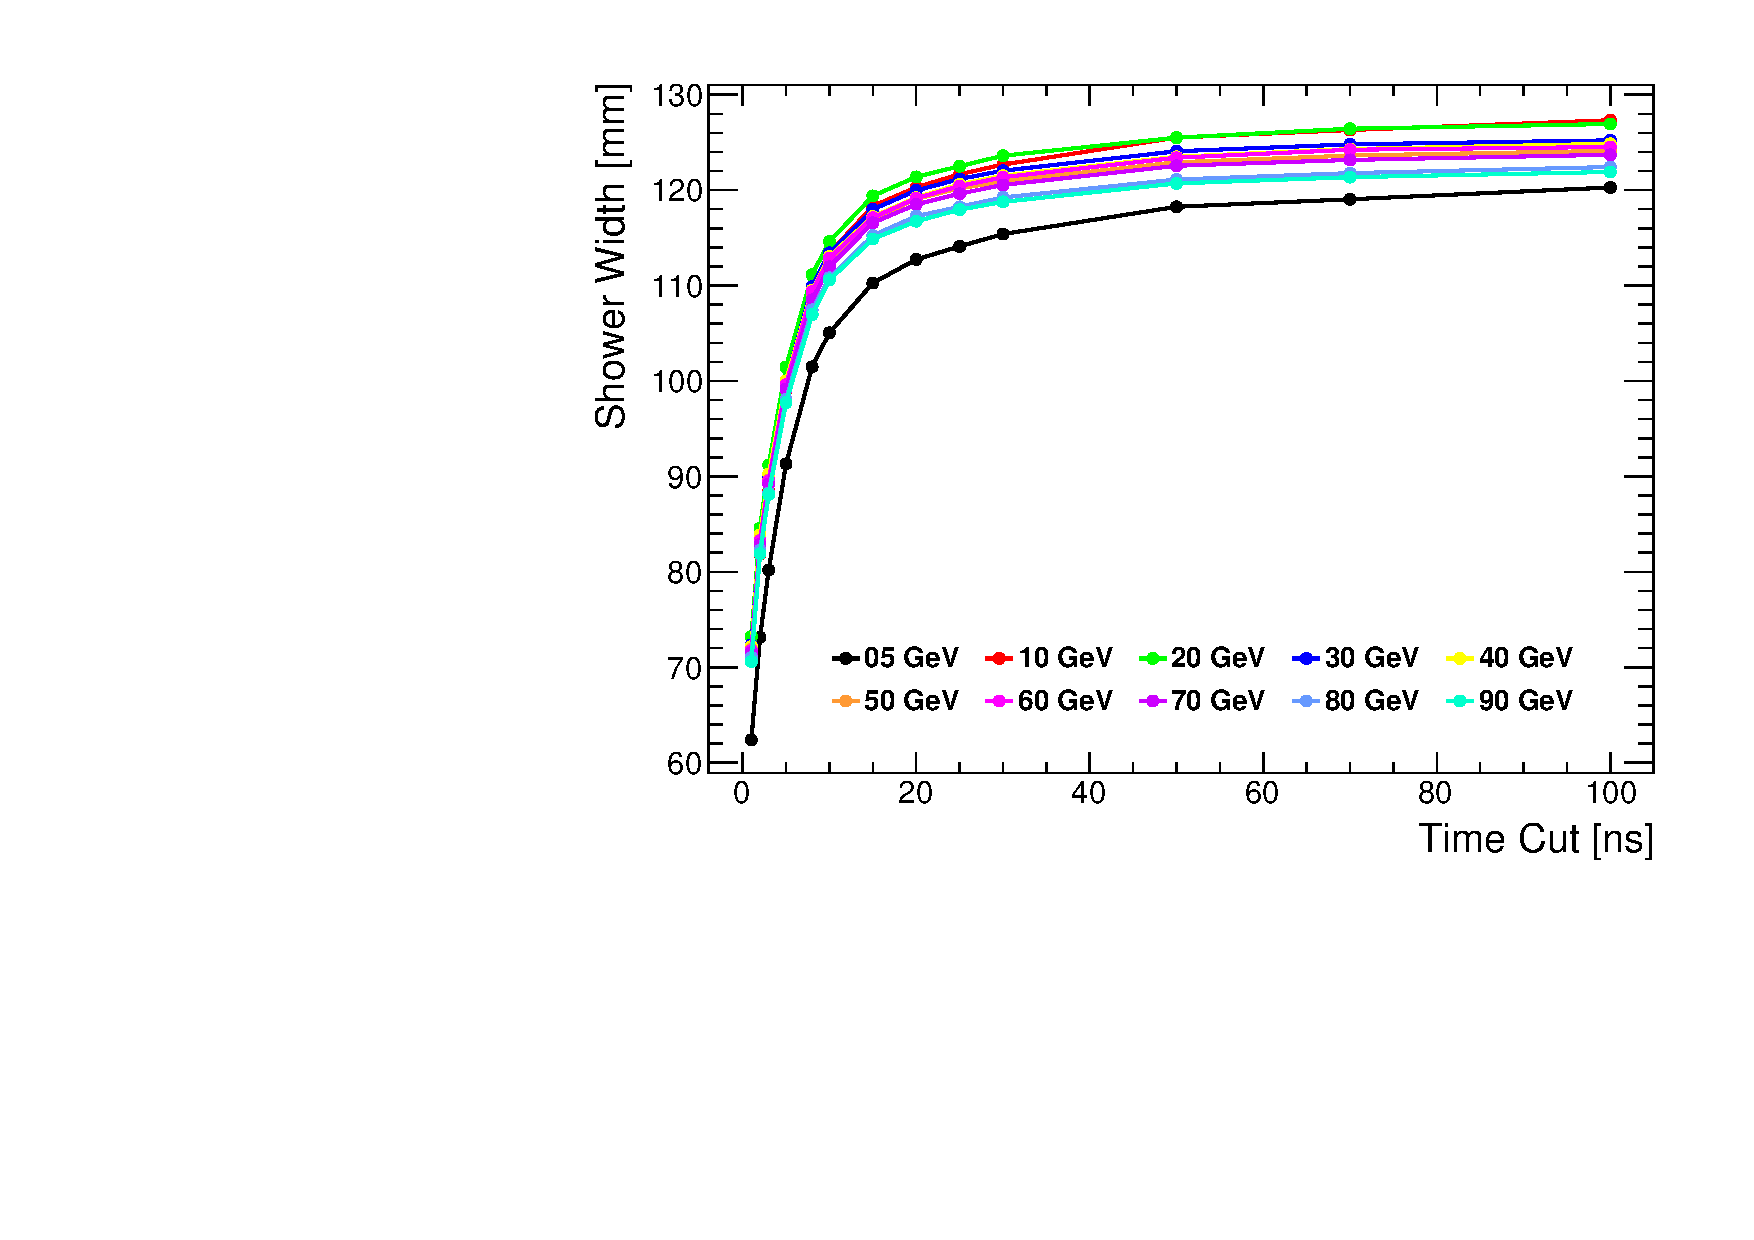
\includegraphics[width=1\linewidth]{chap6/fig_TimingILD/NoSmearing/ShowerWidthAbso_TimeCuts_noSmearing}
      \caption{} \label{fig:ShowerWidthAbsoNoSmearing}
    \end{subfigure}
  \end{minipage}
  \begin{minipage}{.45\textwidth}
    \centering
    \begin{subfigure}[t]{1\textwidth}
      \centering
      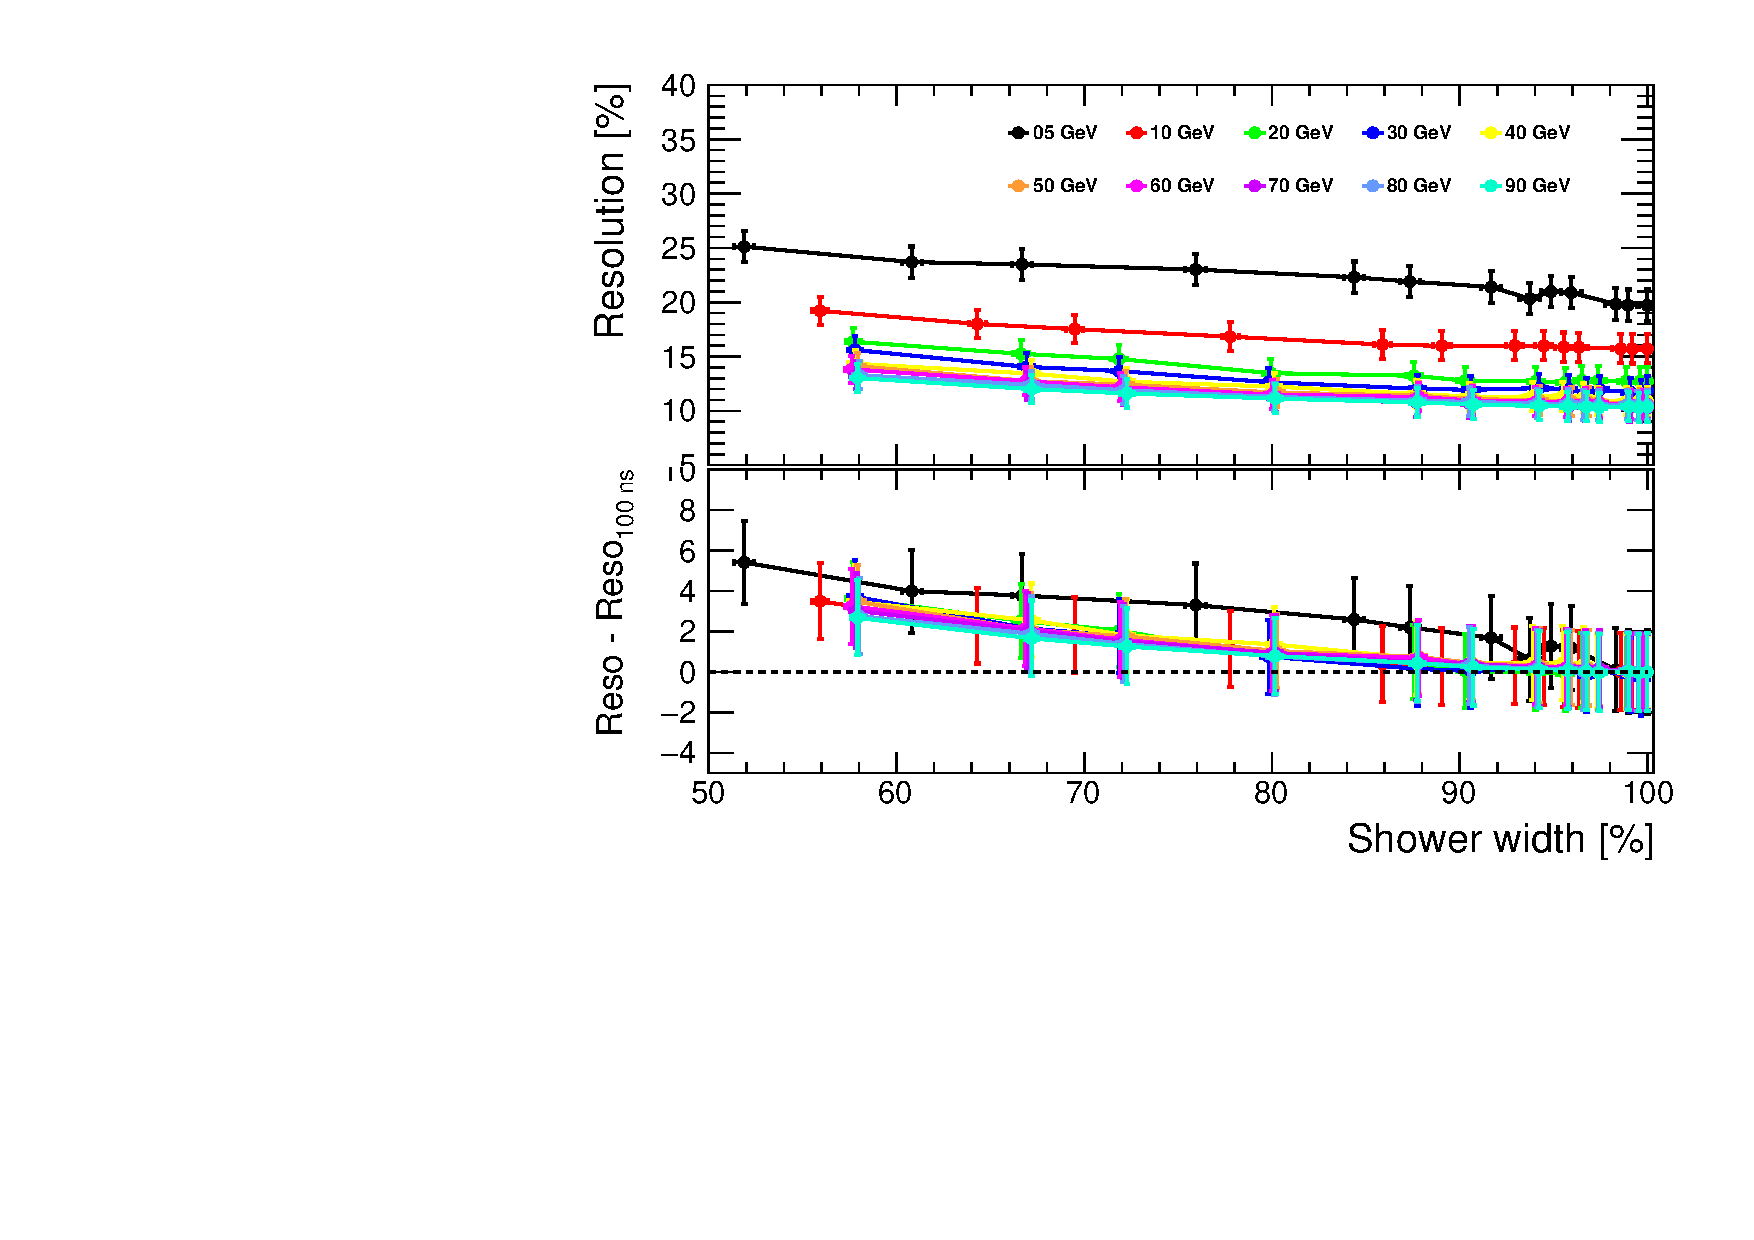
\includegraphics[width=1\linewidth]{chap6/fig_TimingILD/NoSmearing/ShowerWidth_Resolution_noSmearing}
      \vspace{-6ex}
      \caption{}  \label{fig:ShowerWidthResoNoSmearing}
    \end{subfigure}
  \end{minipage}
  \caption{\subref{fig:ShowerWidthNoSmearing}) The plot represents the mean of the shower width <R> as function of timing cut for different particle energies. The y-axis has been normalized to the shower width at \SI{100}{\nano\second}. The shower width decreases steadily as function of the timing cut, indicating that the shower gets narrower. \subref{fig:ShowerWidthAbsoNoSmearing}) The plots represents the absolute value of the mean shower width <R> in \SI{}{\milli\meter} as function of the timing cut. This shows that the low energy showers are generally wider certainly due to the magnetic field. And under \SI{20}{\nano\second}, the width is very similar indicating the core of the shower is fairly similar for all energies. \subref{fig:ShowerWidthResoNoSmearing}) The top plot is the energy resolution as function of shower width for different particle energies. Each point represents a timing cut from \SI{1}{\nano\second} ns to \SI{100}{\nano\second} from left to right. The bottom plot is the loss of resolution compared to the gain in shower width size.}
\end{figure}

It is interresting to look at the gain in the reduction of the shower width compared to the loss in energy resolution. In fact, reducing the shower width would improve the pattern recognition in Pandora. The figure \ref{fig:ShowerWidthResoNoSmearing} shows the resolution loss as function of the shower width. The bottom plots shows the gain in shower width is behaving in the same way for all energies. The tigher the timing cut gets, the small the shower gets as well as a loss in resolution. The main point here is that the gain in shower width is great (up to 60-70\%) compared to the loss in energy resolution (up to 8\%) that could be recovered in a next step after pattern recognition.

This study shows that the use of timing cuts give a great advantage in order to improve pattern recognition without degrading too much the energy resolution of a hadronic shower. However, this study assumes a perfect timing resolution which doesn\'t reflect the reality. In the next section, different time resolution were assumed based on the current knowledge on the timing resolution of the foreseen electronics.

\subsubsection{In a realistic scenario}

In this section, a similar study is performed as in section \ref{}. Instead it assumes realistic time resolutions based on the current electronic technology. The table \ref{table:TimeReso} sums up the investigated time resolutions. The same selection is applied as in the previous section.

\begin{table}[t]
  \centering
  \caption{Time resolution used for smearing.} \label{table:TimeReso}
  \begin{tabular}{|c|c|}
    \hline
    Scenario & Time resolution (ns) \\
    \hline
    Testbeam & 8 \\
    Ideal & 1 \\
    ILC extrapolated & 0.4 \\
    \hline
  \end{tabular}
\end{table}

The testbeam resolution is the time resolution obtained with the current AHCAL technological prototype as explained in section \ref{}. The ideal time resolution is in the order of the time scale of the development of hadronic showers. And finally, the ILC extrapolated is obtained by assuming a linear extrapolation from the tesbeam time resolution with a faster slow clock of \SI{5}{\mega\hertz} instead of \SI{250}{\kilo\hertz} (x20 faster) as explained in \ref{}.\\

\begin{figure}[t]
  \centering
  \begin{minipage}{1\textwidth}
    \begin{subfigure}[t]{0.5\textwidth}
      \centering
      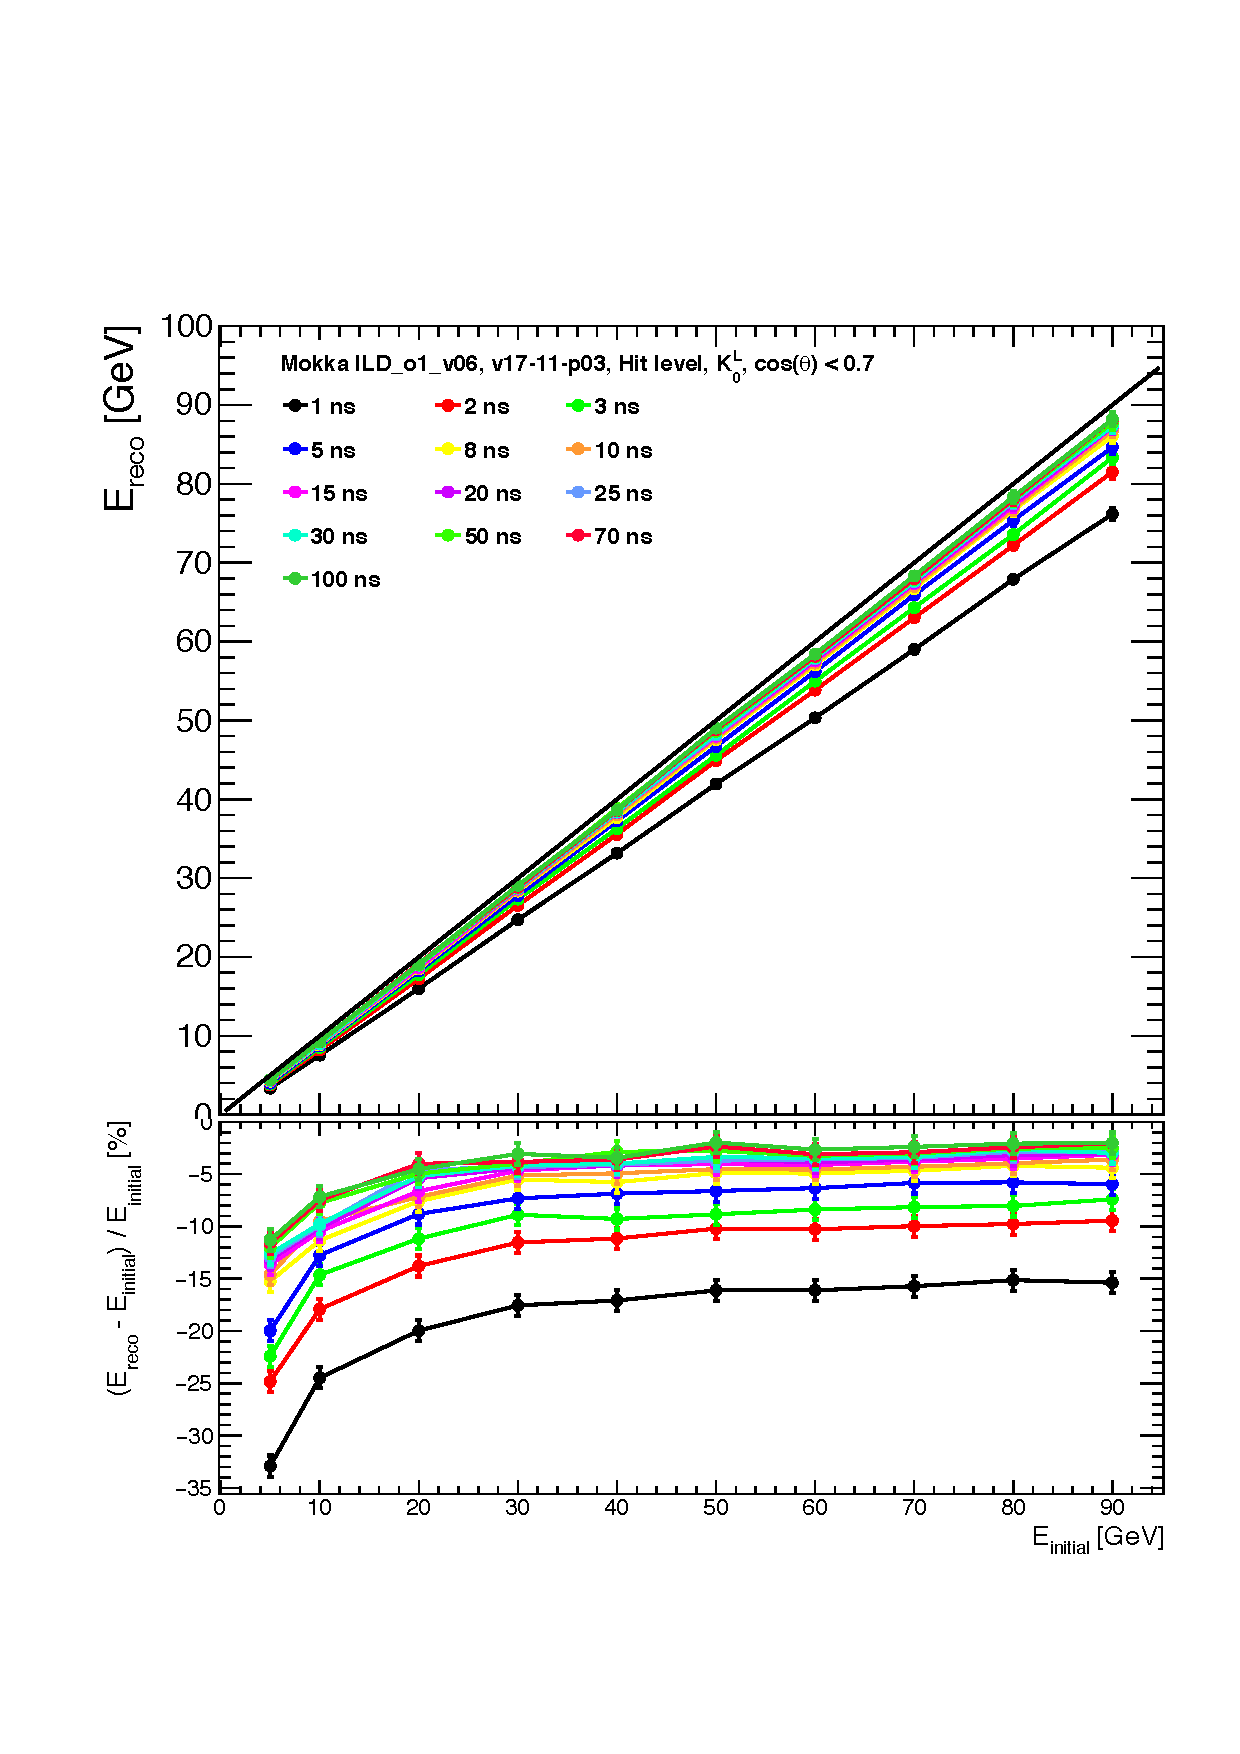
\includegraphics[width=1\linewidth]{chap6/fig_TimingILD/0.4ns_Smearing/Linearity_TimeCuts_Smearing0.4ns}
      \vspace{-6ex}
      \caption{\SI{0.4}{\nano\second} time smearing.} \label{fig:Lin0.4ns}
    \end{subfigure}
    \begin{subfigure}[t]{0.5\textwidth}
      \centering
      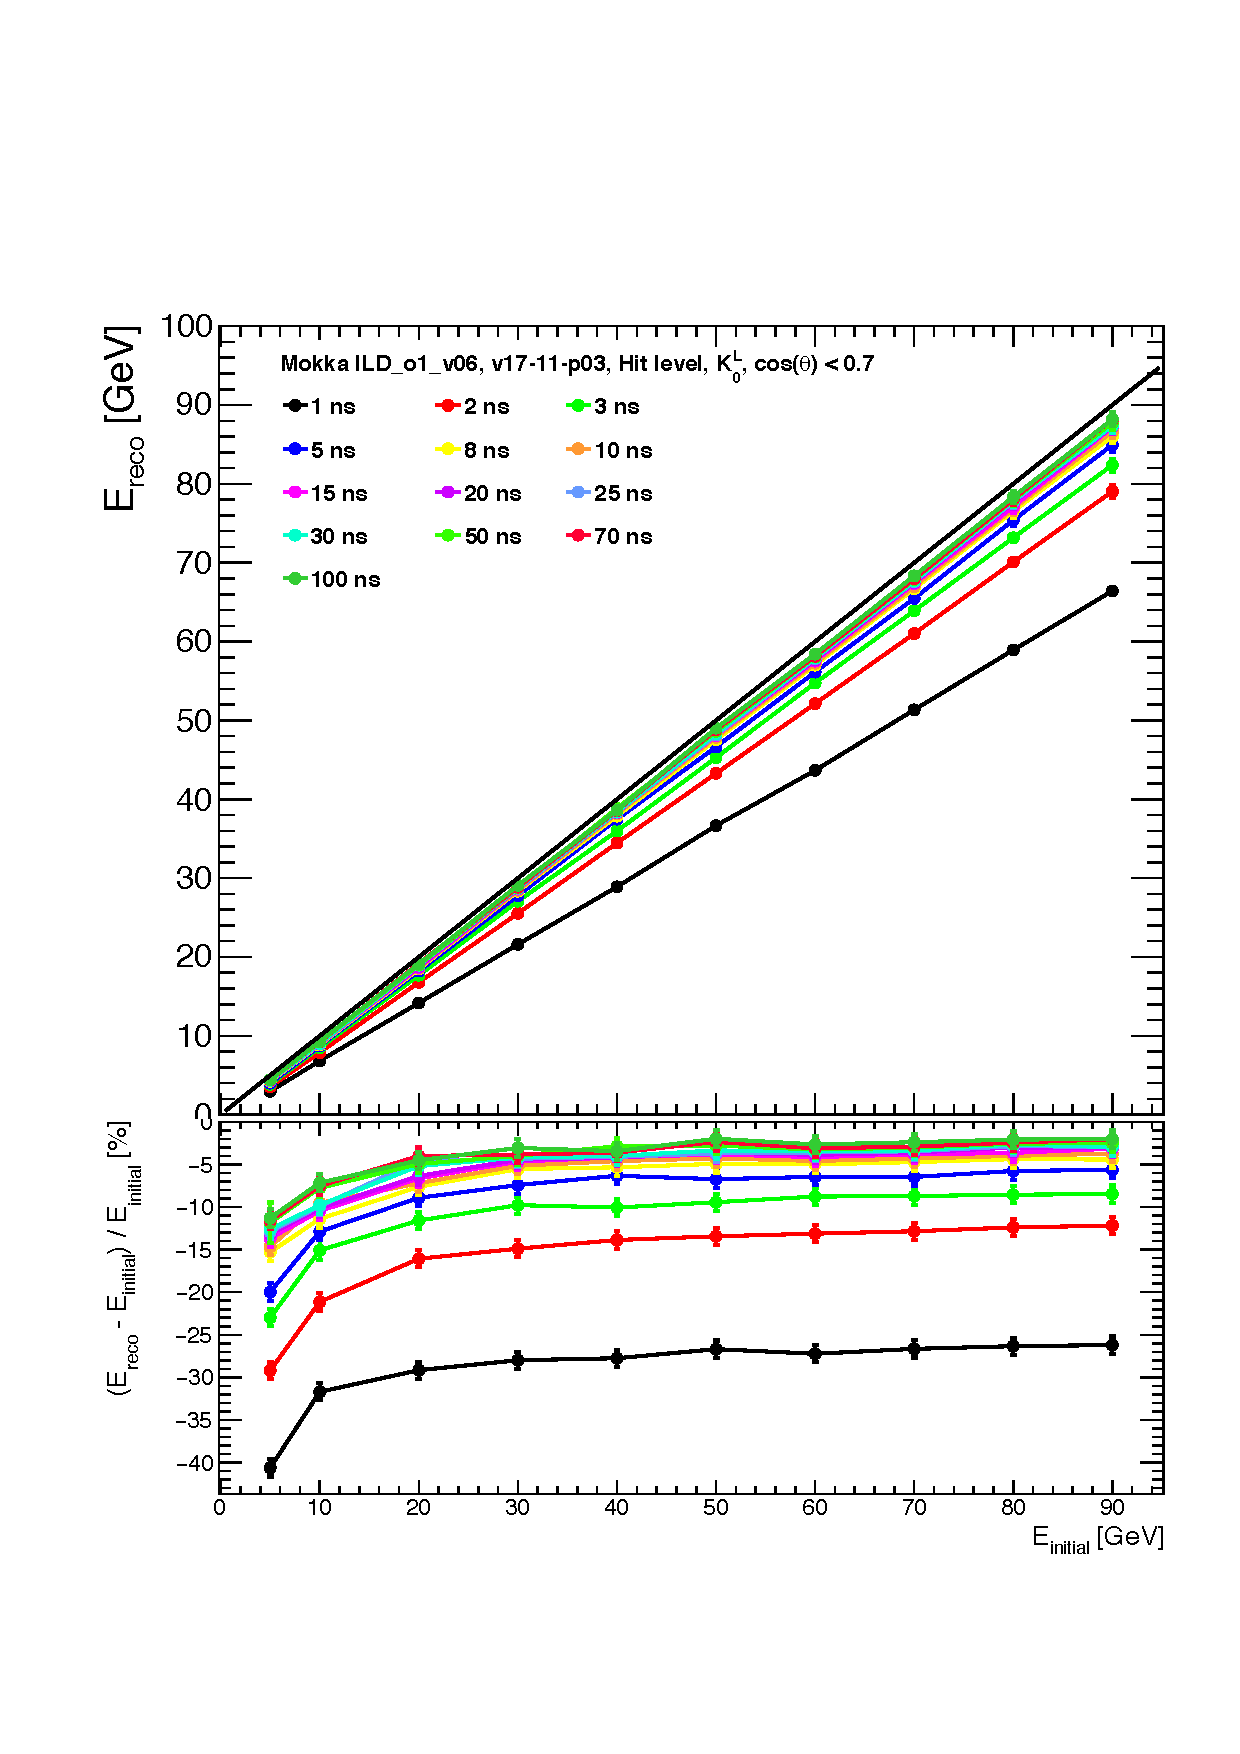
\includegraphics[width=1\linewidth]{chap6/fig_TimingILD/1ns_Smearing/Linearity_TimeCuts_Smearing1ns}
      \vspace{-6ex}
      \caption{\SI{1}{\nano\second} time smearing.} \label{fig:Lin1ns}
    \end{subfigure}
  \end{minipage}
  \begin{subfigure}[t]{0.5\textwidth}
    \centering
    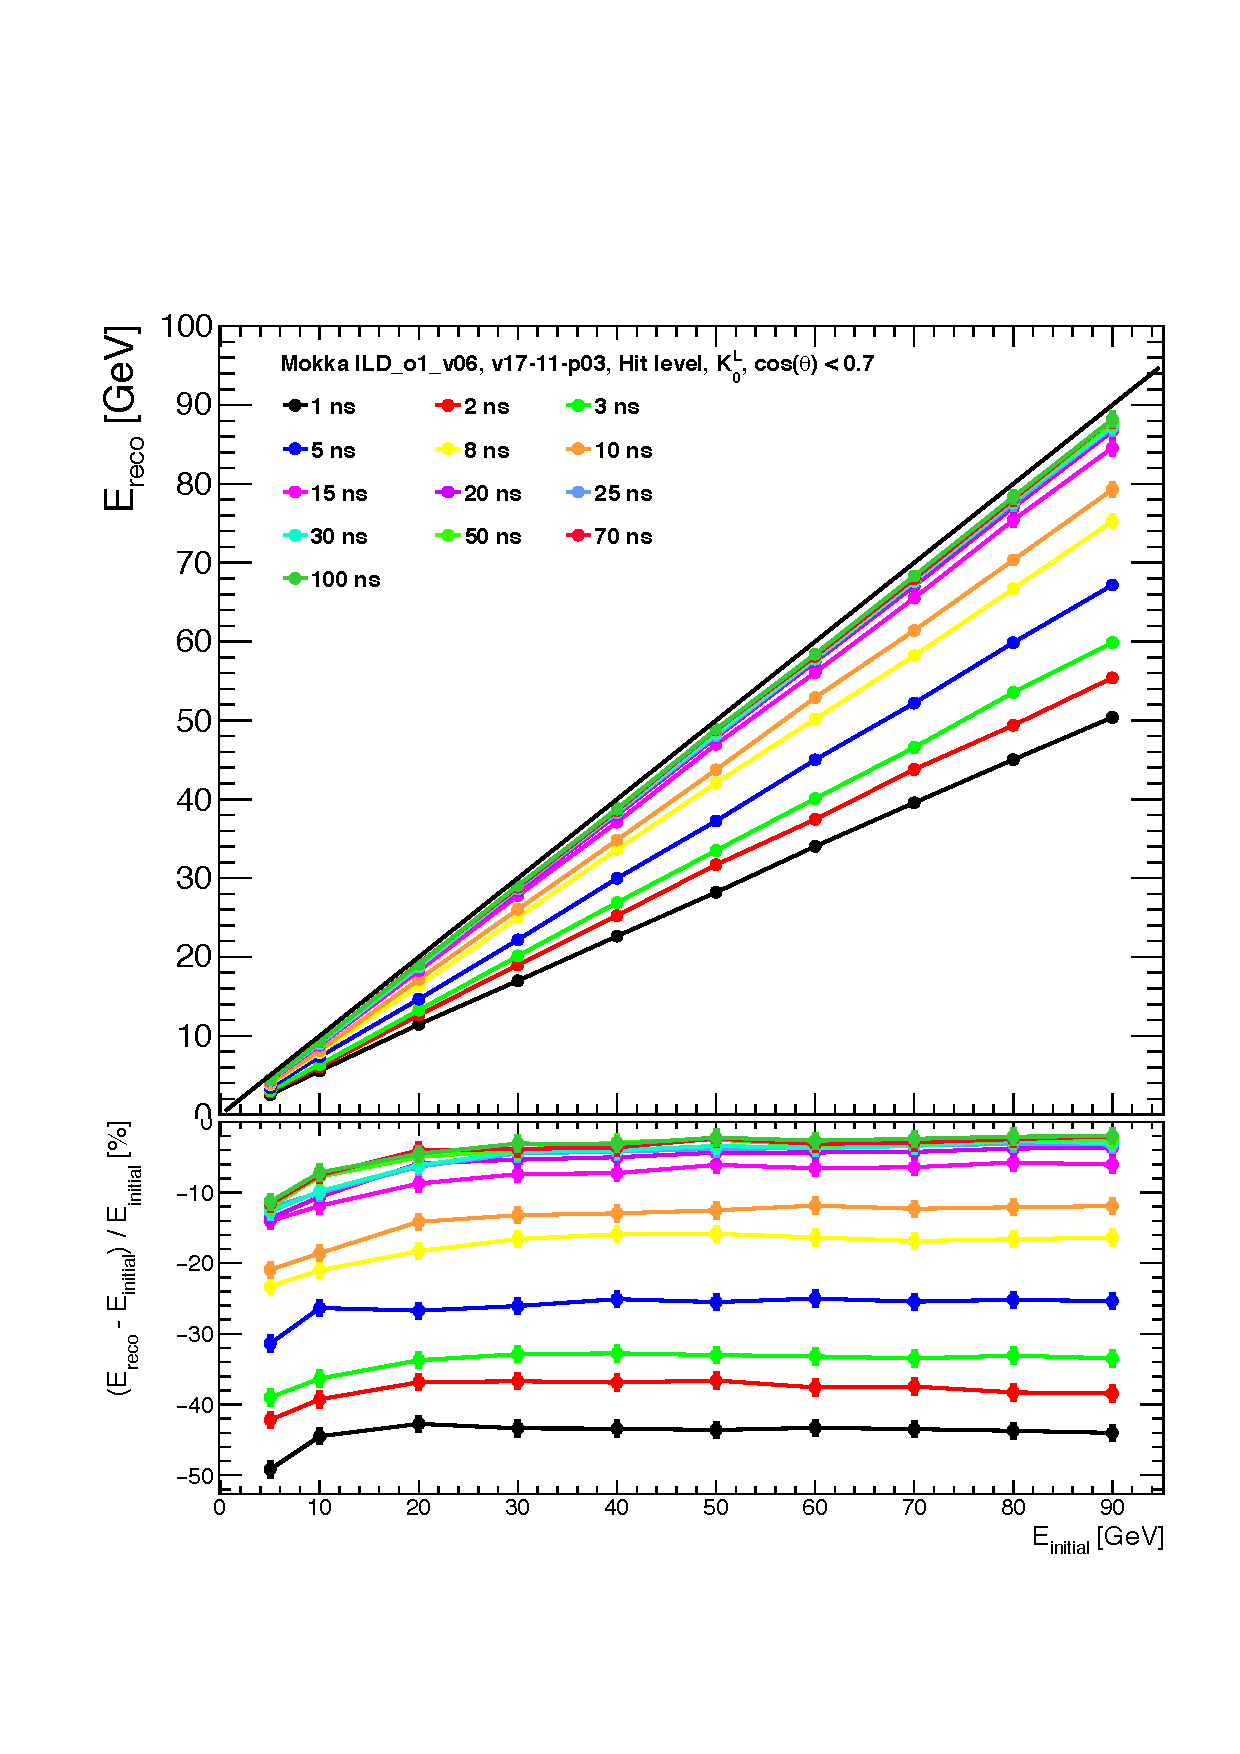
\includegraphics[width=1\linewidth]{chap6/fig_TimingILD/8ns_Smearing/Linearity_TimeCuts_Smearing8ns}
    \vspace{-6ex}
    \caption{\SI{8}{\nano\second} time smearing.}  \label{fig:Lin8ns}
  \end{subfigure}
  \caption{Linearity curves for different assumed time resolutions (0.4 to 8 ns from left to right). The top plot represents the mean reconstructed energy $E_{reco}$ for kaons from 5 to 90 \GeV. The bottom plot shows the relative deviation to the line $x=y$.}
\end{figure}

Looking at the impact on linearity and energy resolution, time resolution in the order of sub-nanosecond does not affect much the linearity and resolution as shown in figures \ref{fig:Lin0.4ns} and \ref{fig:Reso0.4ns}. For a time resolution in the nanosecond order, the figures \ref{fig:Lin1ns} and \ref{fig:Reso1ns} show that a tight timing cut of 1-2 \SI{}{\nano\second} will start to affect linearity and resolution. However, for timing resolution higher, the linearity and resolution, as shown in figures \ref{fig:Lin8ns} and \ref{fig:Reso8ns}, start to get heavily degraded for timing cuts below 10-20 \SI{}{\nano\second}. This tells that at least a time resolution of around \SI{1}{\nano\second} is needed in order to use time information without impacting calorimeter performance too much.

\begin{figure}[t]
  \centering
  \begin{minipage}{1\textwidth}
    \begin{subfigure}[t]{0.5\textwidth}
      \centering
      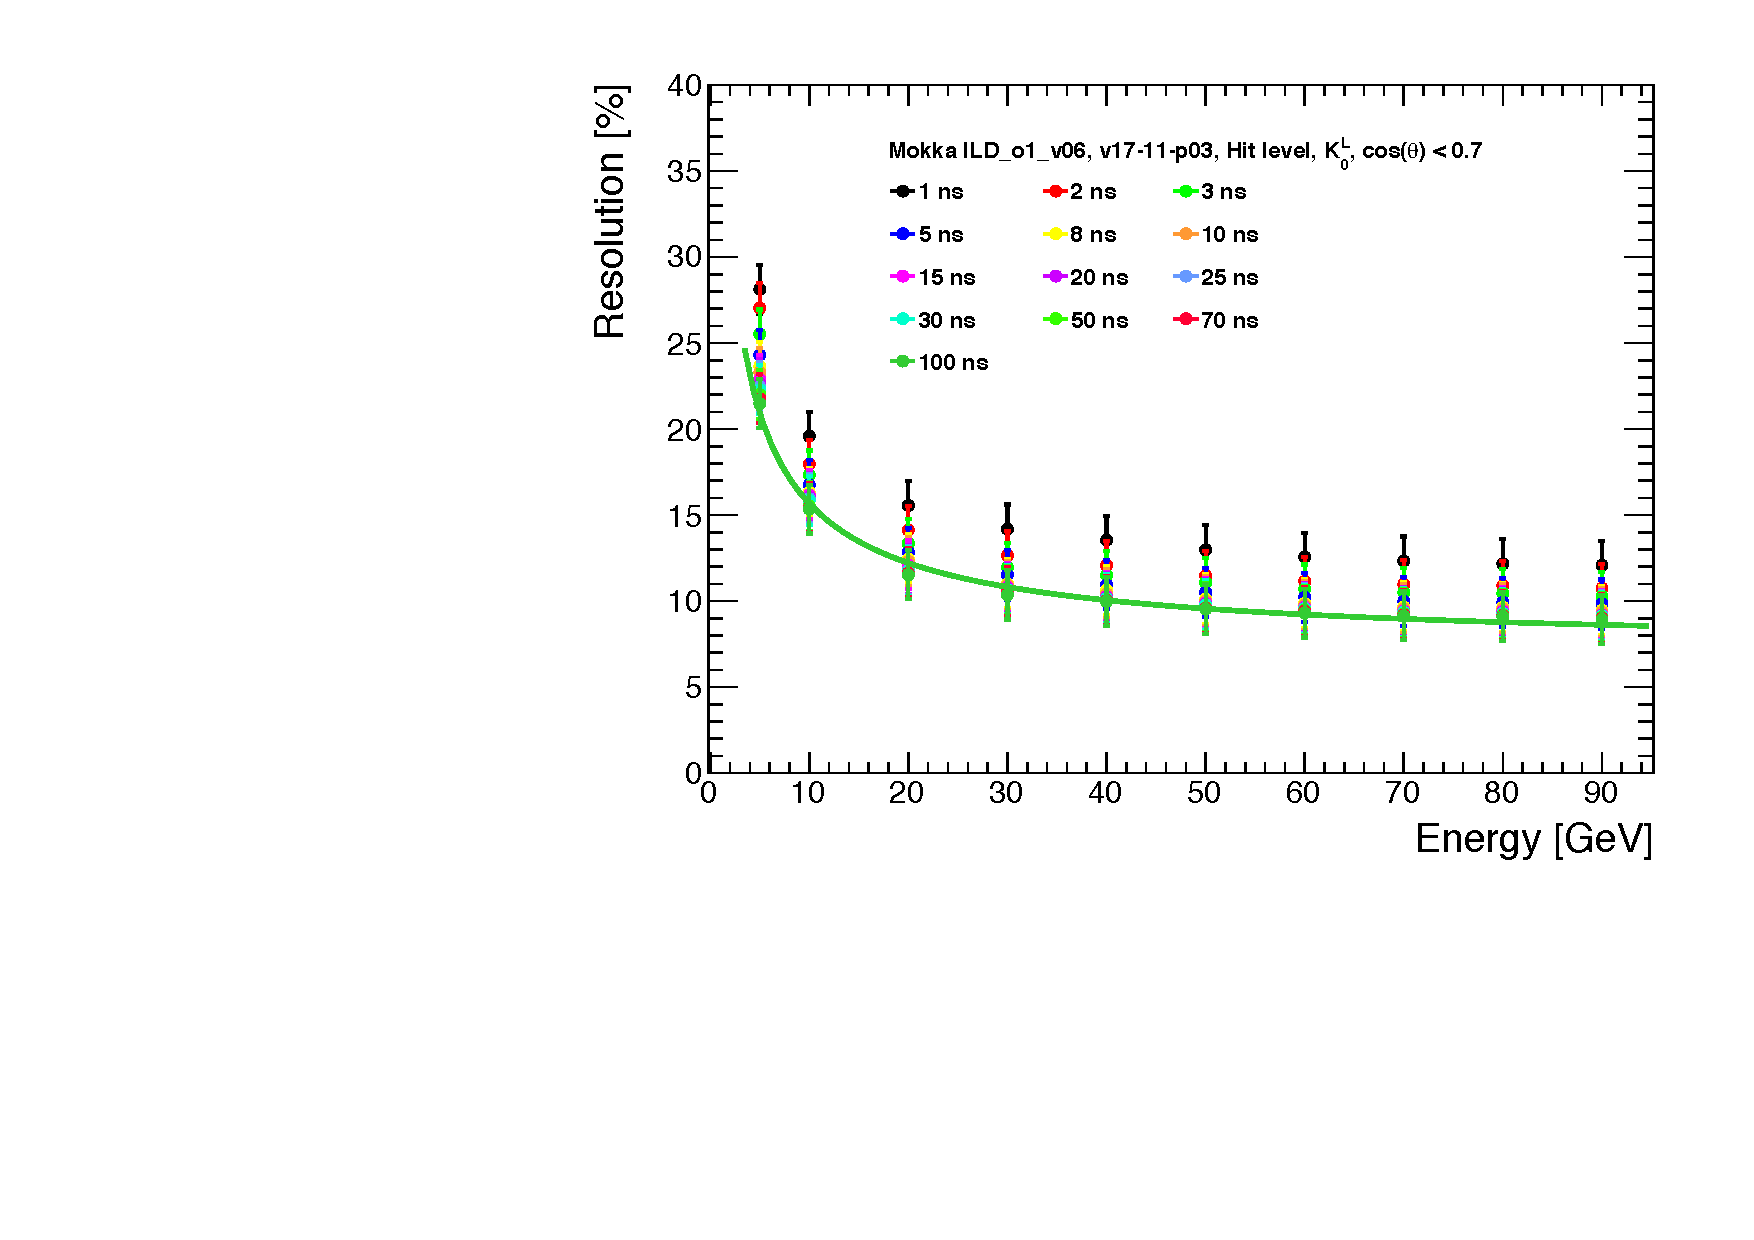
\includegraphics[width=1\linewidth]{chap6/fig_TimingILD/0.4ns_Smearing/ShowerResoAbsolute_TimeCuts_Smearing0.4ns}
      \caption{\SI{0.4}{\nano\second} time smearing.} \label{fig:Reso0.4ns}
    \end{subfigure}
    \begin{subfigure}[t]{0.5\textwidth}
      \centering
      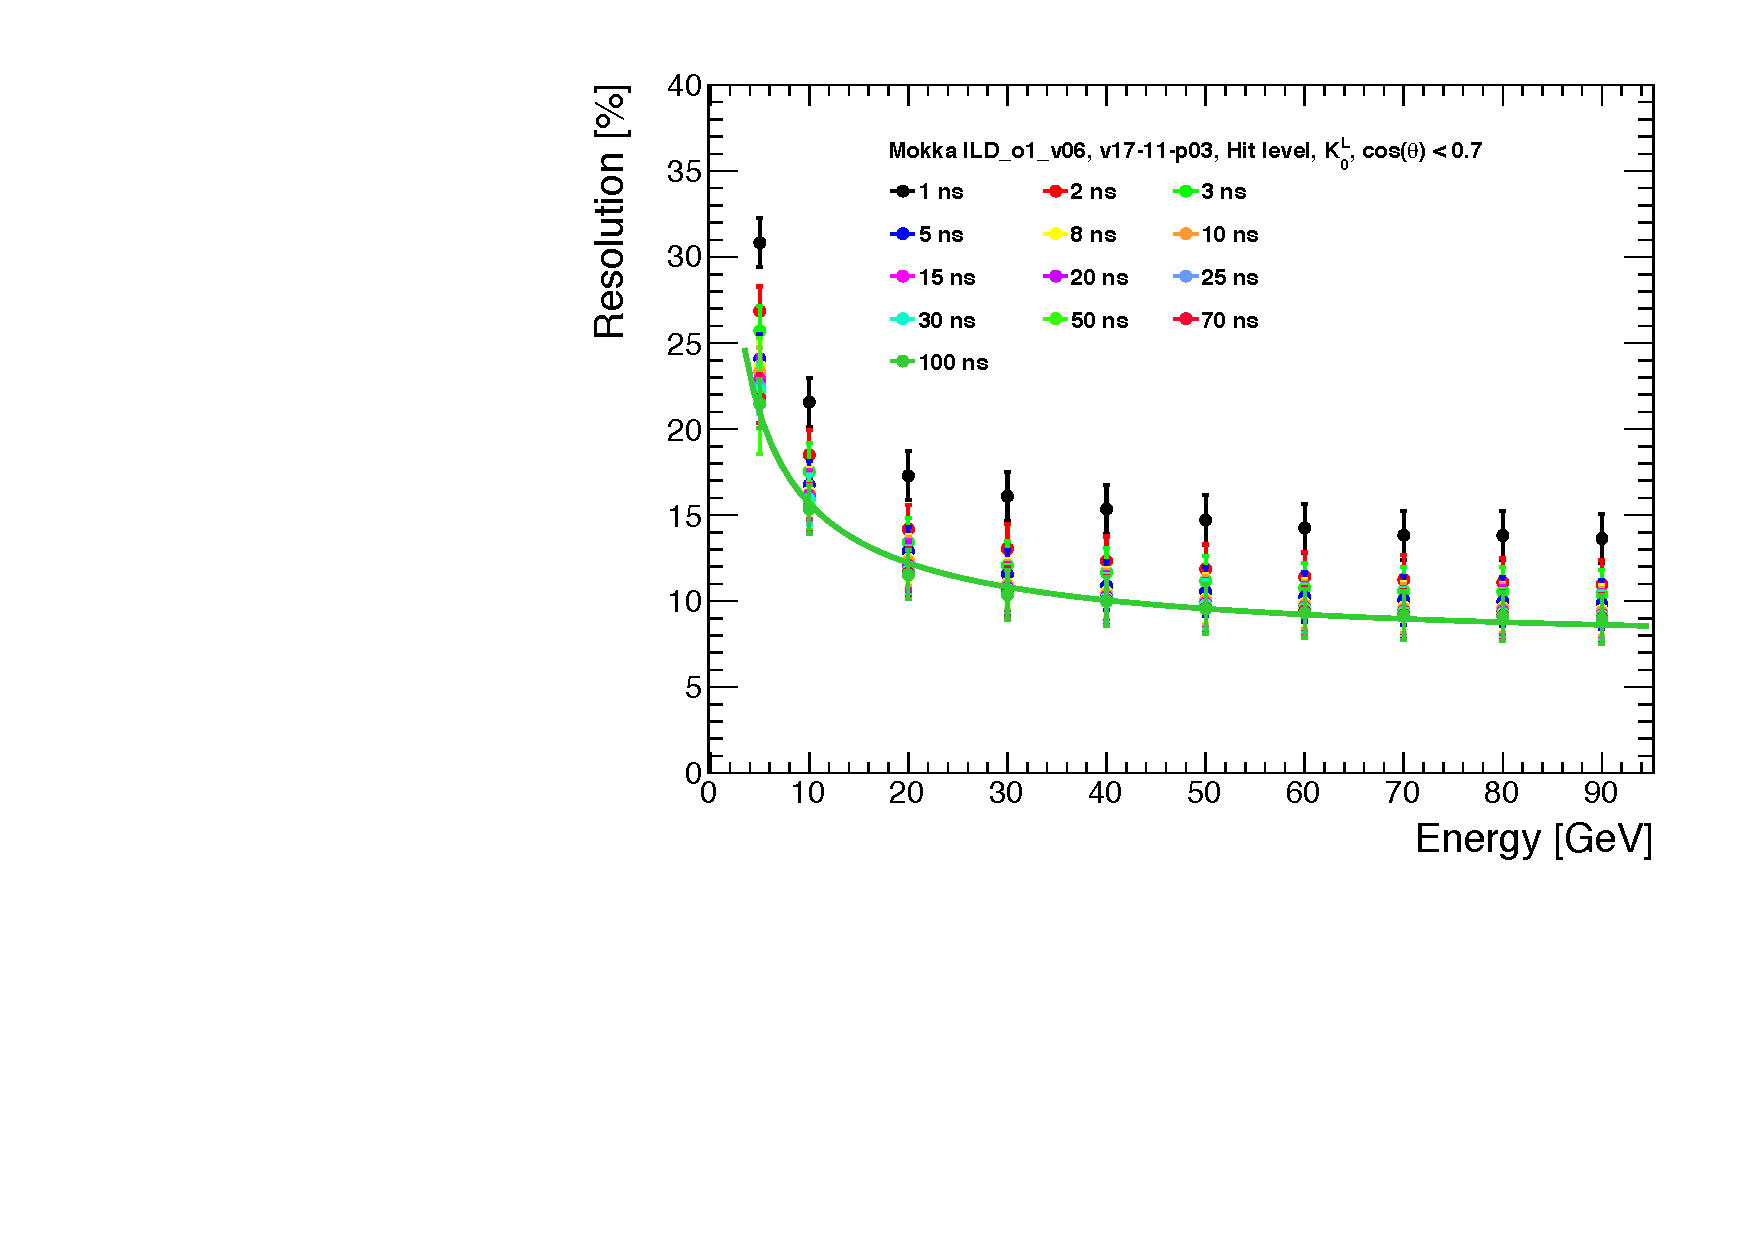
\includegraphics[width=1\linewidth]{chap6/fig_TimingILD/1ns_Smearing/ShowerResoAbsolute_TimeCuts_Smearing1ns}
      \caption{\SI{1}{\nano\second} time smearing.} \label{fig:Reso1ns}
    \end{subfigure}
  \end{minipage}
  \begin{subfigure}[t]{0.5\textwidth}
    \centering
    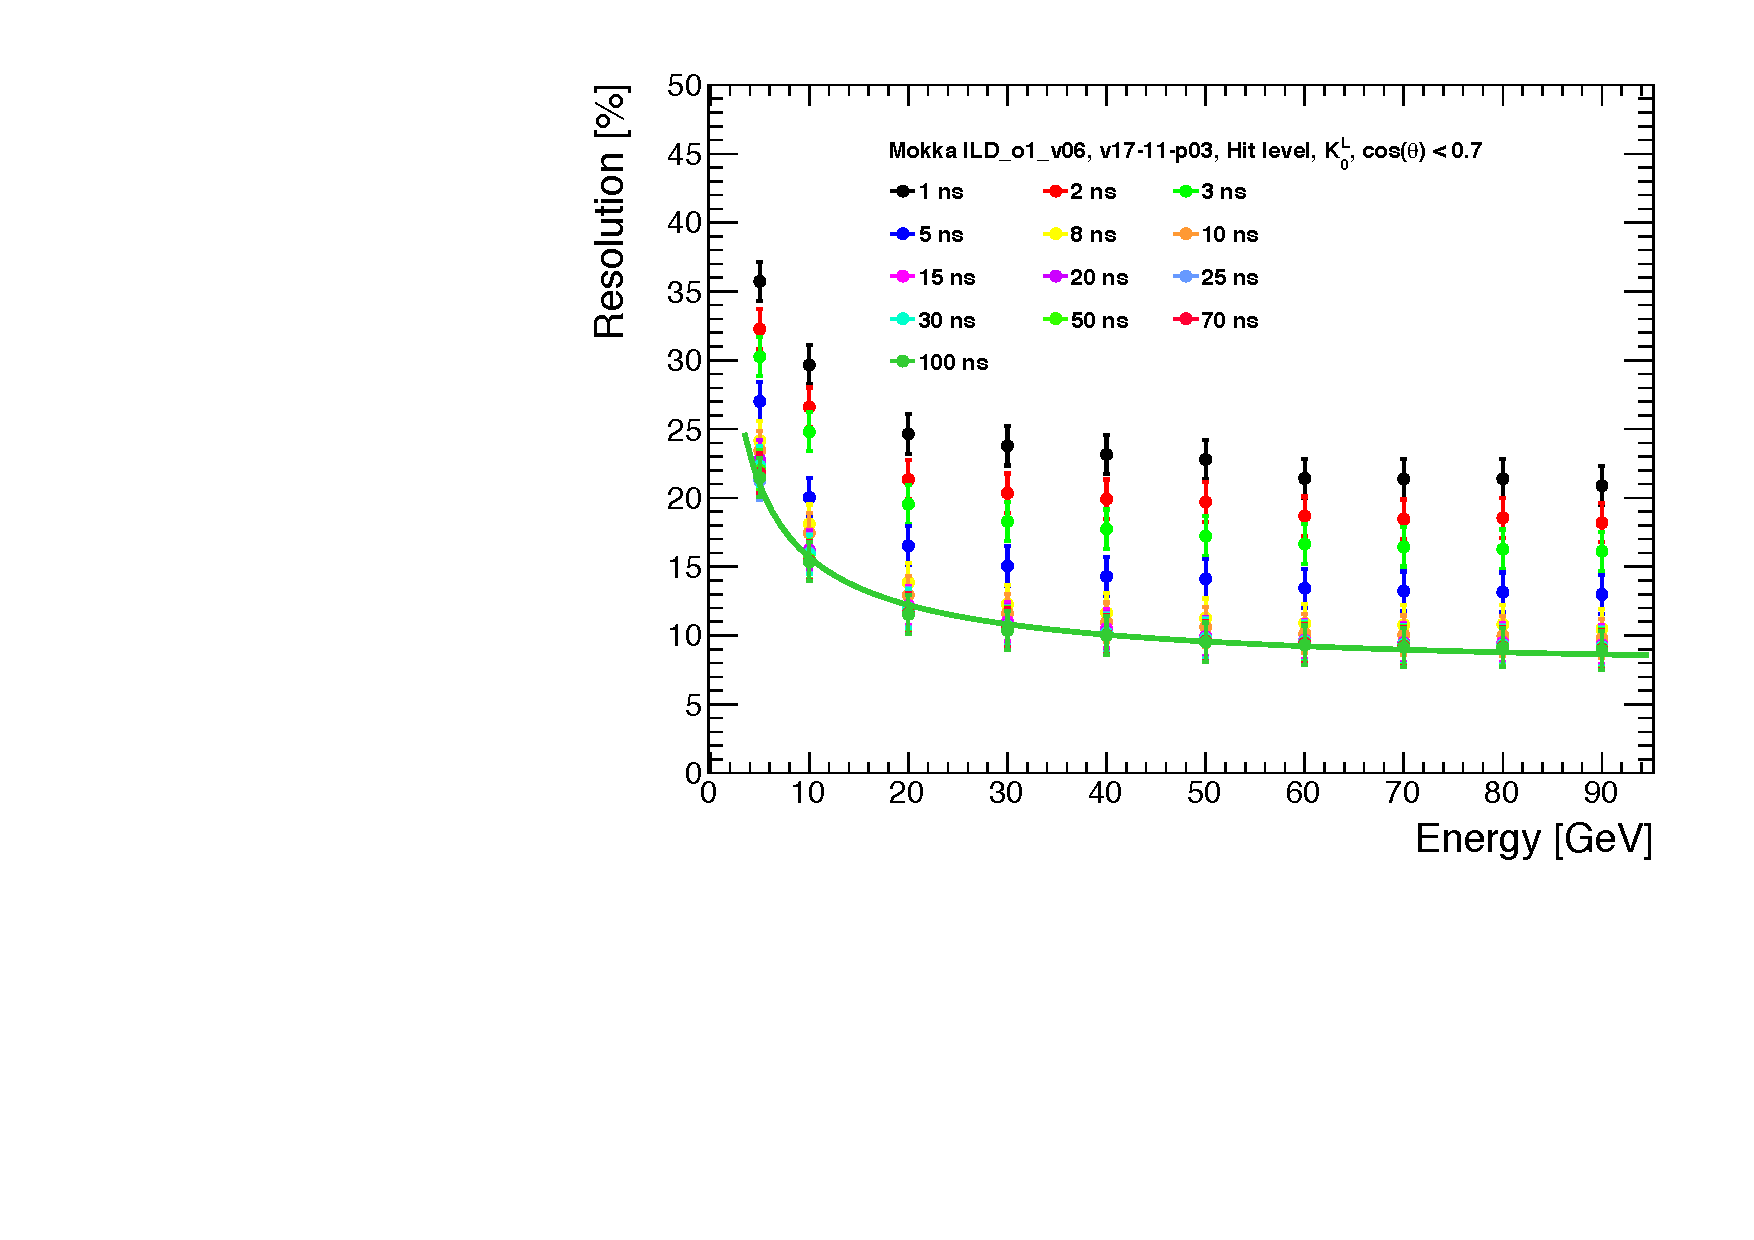
\includegraphics[width=1\linewidth]{chap6/fig_TimingILD/8ns_Smearing/ShowerResoAbsolute_TimeCuts_Smearing8ns}
    \caption{\SI{8}{\nano\second} time smearing.}  \label{fig:Reso8ns}
  \end{subfigure}
  \caption{Energy resolution curves for different assumed time resolutions (0.4 to 8 ns from left to right). The plot represents the relative energy resolution $\frac{\sigma_{E}}{E}$ for kaons from 5 to 90 \GeV for each timing cut. The green line is a fit applied to 100 ns timing cut of the typical form $\frac{\sigma_{E}}{E} = \frac{a}{\sqrt{E}} \bigoplus b$.}
\end{figure}

\begin{figure}[t]
  \centering
  \begin{minipage}{1\textwidth}
    \begin{subfigure}[t]{0.5\textwidth}
      \centering
      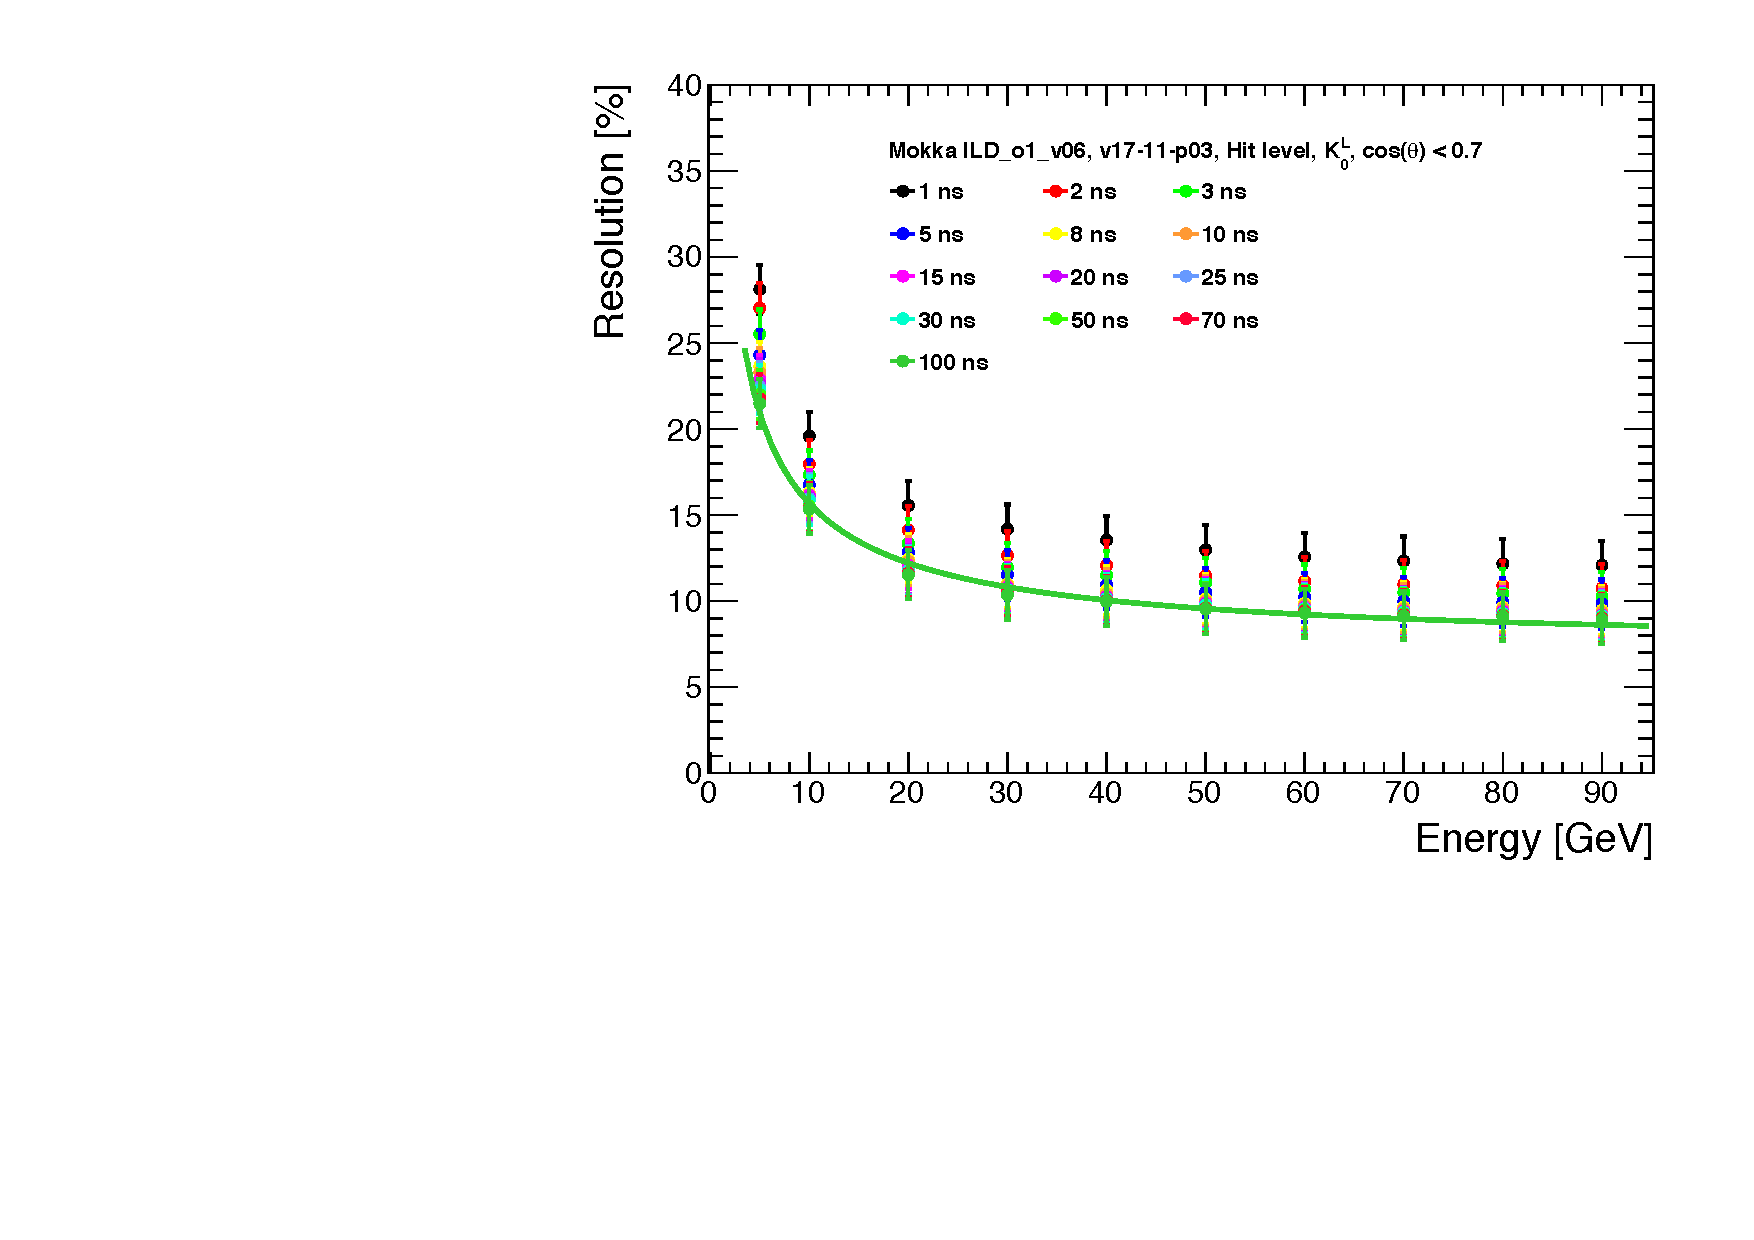
\includegraphics[width=1\linewidth]{chap6/fig_TimingILD/0.4ns_Smearing/ShowerResoAbsolute_TimeCuts_Smearing0.4ns}
      \caption{\SI{0.4}{\nano\second} time smearing.} \label{fig:Reso0.4ns}
    \end{subfigure}
    \begin{subfigure}[t]{0.5\textwidth}
      \centering
      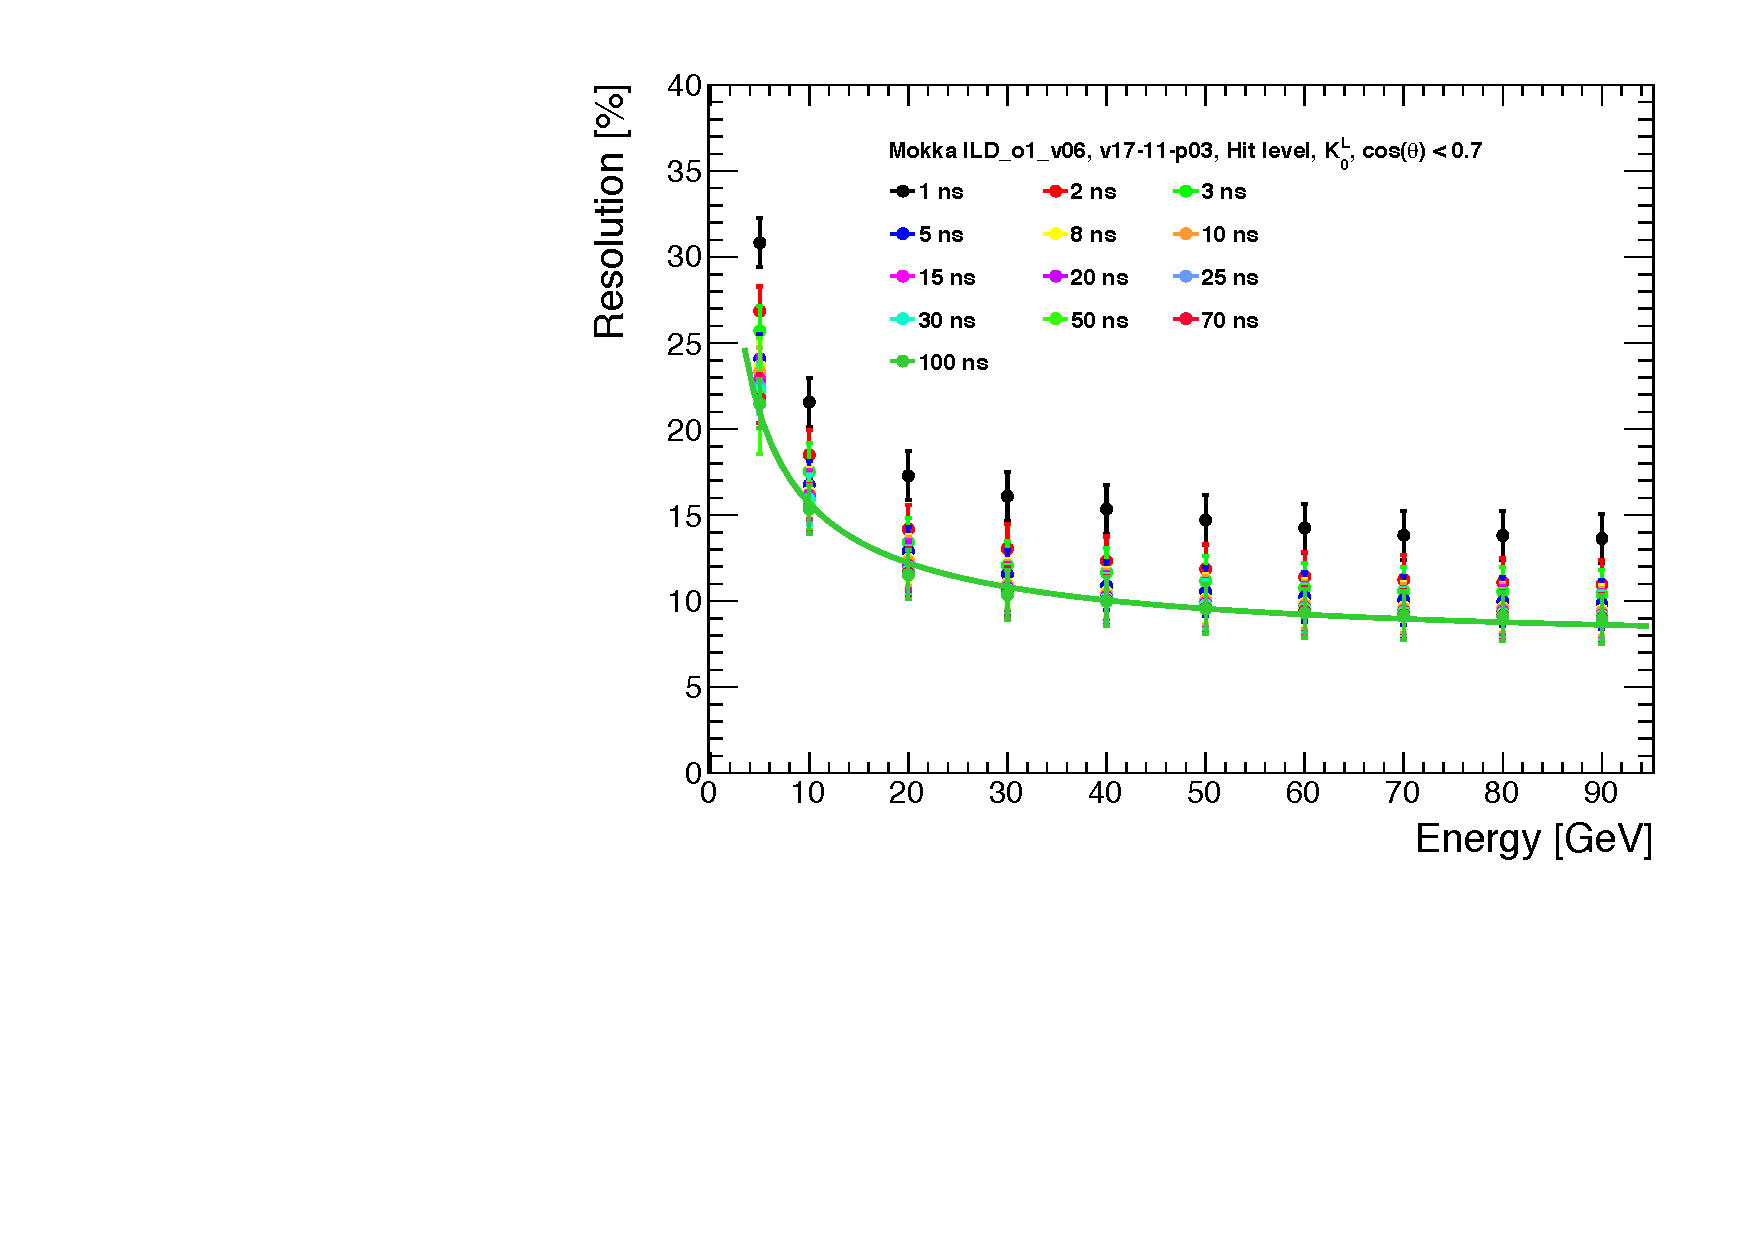
\includegraphics[width=1\linewidth]{chap6/fig_TimingILD/1ns_Smearing/ShowerResoAbsolute_TimeCuts_Smearing1ns}
      \caption{\SI{1}{\nano\second} time smearing.} \label{fig:Reso1ns}
    \end{subfigure}
  \end{minipage}
  \begin{subfigure}[t]{0.5\textwidth}
    \centering
    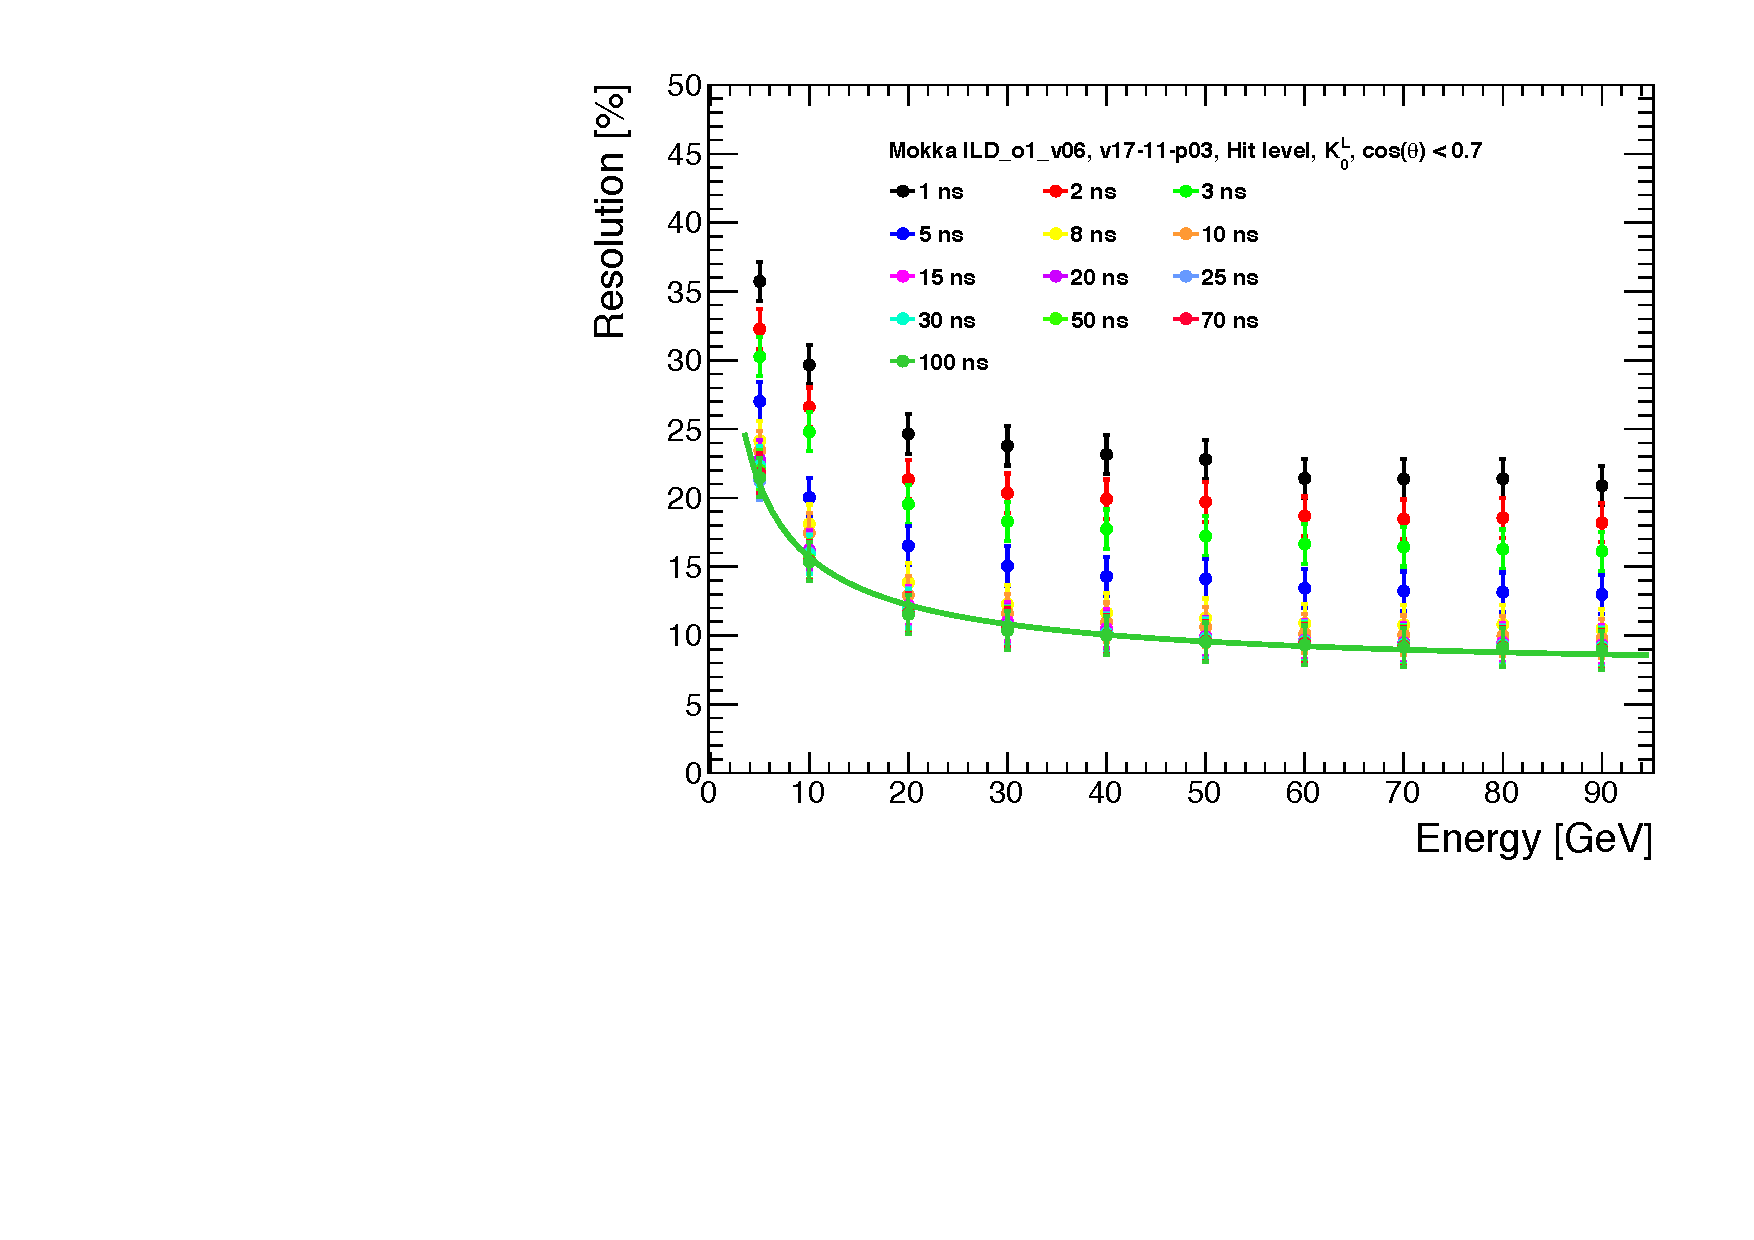
\includegraphics[width=1\linewidth]{chap6/fig_TimingILD/8ns_Smearing/ShowerResoAbsolute_TimeCuts_Smearing8ns}
    \caption{\SI{8}{\nano\second} time smearing.}  \label{fig:Reso8ns}
  \end{subfigure}
  \caption{Energy resolution curves for different assumed time resolutions (0.4 to 8 ns from left to right). The plot represents the relative energy resolution $\frac{\sigma_{E}}{E}$ for kaons from 5 to 90 \GeV for each timing cut. The green line is a fit applied to 100 ns timing cut of the typical form $\frac{\sigma_{E}}{E} = \frac{a}{\sqrt{E}} \bigoplus b$.}
\end{figure}

\section{Benchmarking of fast simulation}

\subsection{SGV: fast simulation software}
\subsection{Particle Flow parametrisation}
\subsection{Benchmarking against full ILD Simulation}
